%% Springer Nature (sn-jnl) version for Empirical Software Engineering.
%% GENERATED by experiments/build_ese.py from manuscript/latex/*.tex --
%% edit the sources there (or this template), not main.tex.
\documentclass[pdflatex,sn-basic]{sn-jnl}

\usepackage{graphicx}%
\usepackage{multirow}%
\usepackage{amsmath,amssymb,amsfonts}%
\usepackage{amsthm}%
\usepackage{mathrsfs}%
\usepackage{xcolor}%
\usepackage{textcomp}%
\usepackage{manyfoot}%
\usepackage{booktabs}%
\usepackage{algorithm}%
\usepackage{algorithmicx}%
\usepackage{algpseudocode}%
\usepackage{tikz}%
\usetikzlibrary{positioning,arrows.meta,fit,calc,backgrounds}%
\usepackage{url}%
\usepackage{adjustbox}%
%% sn-jnl's table rules use a brace-counting trick that breaks inside boxes;
%% plain rules are used instead so wide tables can be scaled to the text width.
\let\toprule\hline\let\midrule\hline\let\bottomrule\hline\let\botrule\hline
\renewcommand{\arraystretch}{1.15}

\theoremstyle{thmstyleone}%
\newtheorem{proposition}{Proposition}%
\raggedbottom

\newcommand{\cBvGgnnAnonVLexD}{+0.202}
\newcommand{\cBvGgnnAnonVLexHi}{+0.249}
\newcommand{\cBvGgnnAnonVLexLo}{+0.149}
\newcommand{\cBvGgnnAnonVLexSsD}{+0.102}
\newcommand{\cBvGgnnAnonVLexSsHi}{+0.144}
\newcommand{\cBvGgnnAnonVLexSsLo}{+0.024}
\newcommand{\cBvGgnnKindLowVKindD}{+0.017}
\newcommand{\cBvGgnnKindLowVKindHi}{+0.040}
\newcommand{\cBvGgnnKindLowVKindLo}{+0.004}
\newcommand{\cBvGgnnKindVAnonD}{-0.017}
\newcommand{\cBvGgnnKindVAnonHi}{+0.012}
\newcommand{\cBvGgnnKindVAnonKindD}{-0.010}
\newcommand{\cBvGgnnKindVAnonKindHi}{+0.014}
\newcommand{\cBvGgnnKindVAnonKindLo}{-0.038}
\newcommand{\cBvGgnnKindVAnonLo}{-0.050}
\newcommand{\cBvGgnnKindVLexD}{+0.185}
\newcommand{\cBvGgnnKindVLexH}{$<0.001$}
\newcommand{\cBvGgnnKindVLexHi}{+0.236}
\newcommand{\cBvGgnnKindVLexKindD}{+0.100}
\newcommand{\cBvGgnnKindVLexKindHi}{+0.156}
\newcommand{\cBvGgnnKindVLexKindLo}{+0.064}
\newcommand{\cBvGgnnKindVLexLo}{+0.130}
\newcommand{\cBvGgnnKindVLexNoAnd}{+0.194 [+0.127, +0.241]}
\newcommand{\cBvGgnnKindVLexP}{$<0.001$}
\newcommand{\cBvGgnnKindVLexSsD}{+0.069}
\newcommand{\cBvGgnnKindVLexSsHi}{+0.112}
\newcommand{\cBvGgnnKindVLexSsLo}{-0.014}
\newcommand{\cBvGgnnKindVLexW}{0.002}
\newcommand{\cBvGgnnKindVLexWH}{0.225}
\newcommand{\cBvGgnnKindVLexWblk}{0.062}
\newcommand{\cBvGgnnKindVLexWins}{10/10}
\newcommand{\cBvGgnnKindVLinevulNormD}{-0.037}
\newcommand{\cBvGgnnKindVLinevulNormHi}{-0.018}
\newcommand{\cBvGgnnKindVLinevulNormLo}{-0.068}
\newcommand{\cBvGgnnKindVOpD}{+0.042}
\newcommand{\cBvGgnnKindVOpHi}{+0.067}
\newcommand{\cBvGgnnKindVOpLo}{-0.004}
\newcommand{\cBvGgnnKindVSizeD}{-0.045}
\newcommand{\cBvGgnnKindVSizeHi}{-0.022}
\newcommand{\cBvGgnnKindVSizeLo}{-0.086}
\newcommand{\cBvGgnnKindVUnixNormD}{+0.047}
\newcommand{\cBvGgnnKindVUnixNormHi}{+0.091}
\newcommand{\cBvGgnnKindVUnixNormLo}{+0.003}
\newcommand{\cBvGgnnLexKindVLexD}{+0.086}
\newcommand{\cBvGgnnLexKindVLexHi}{+0.111}
\newcommand{\cBvGgnnLexKindVLexLo}{+0.038}
\newcommand{\cBvGgnnOpKindVKindD}{-0.004}
\newcommand{\cBvGgnnOpKindVKindHi}{+0.021}
\newcommand{\cBvGgnnOpKindVKindLo}{-0.017}
\newcommand{\cBvGgnnOpKindVKindW}{1.000}
\newcommand{\cBvGgnnOpVLexD}{+0.143}
\newcommand{\cBvGinOpKindVKindD}{+0.015}
\newcommand{\cDvGatKindVLexD}{+0.094}
\newcommand{\cDvGgnnKindVAnonKindD}{-0.012}
\newcommand{\cDvGgnnKindVAnonKindHi}{+0.002}
\newcommand{\cDvGgnnKindVAnonKindLo}{-0.030}
\newcommand{\cDvGgnnKindVLexD}{+0.101}
\newcommand{\cDvGgnnKindVLexHi}{+0.132}
\newcommand{\cDvGgnnKindVLexLo}{+0.070}
\newcommand{\cDvGgnnKindVLexSsD}{+0.001}
\newcommand{\cDvGgnnKindVLexSsHi}{+0.039}
\newcommand{\cDvGgnnKindVLexSsLo}{-0.040}
\newcommand{\cDvGgnnKindVLinevulNormD}{-0.038}
\newcommand{\cDvGgnnKindVLinevulNormHi}{-0.023}
\newcommand{\cDvGgnnKindVLinevulNormLo}{-0.056}
\newcommand{\cDvGgnnKindVUnixNormD}{+0.063}
\newcommand{\cDvGgnnOpKindVKindD}{+0.008}
\newcommand{\cDvGgnnOpKindVKindHi}{+0.022}
\newcommand{\cDvGgnnOpKindVKindLo}{-0.005}
\newcommand{\cDvGgnnOpKindVKindW}{0.027}
\newcommand{\cDvGgnnOpKindVKindWins}{8/10}
\newcommand{\cDvGinKindVLexD}{+0.105}
\newcommand{\cDvGinOpKindVKindD}{+0.008}
\newcommand{\mBvGgnnKindLowAuc}{0.708}
\newcommand{\mBvGgnnKindSs}{0.535}
\newcommand{\mBvGgnnLexAuc}{0.506}
\newcommand{\mBvGgnnLexKindAuc}{0.592}
\newcommand{\mBvGgnnLexSs}{0.467}
\newcommand{\mBvTfKindAuc}{0.706}
\newcommand{\mBvTfLexAuc}{0.582}
\newcommand{\mDvGgnnKindSs}{0.523}
\newcommand{\mDvGgnnLexAuc}{0.566}
\newcommand{\mDvGgnnLexKindAuc}{0.607}
\newcommand{\mDvGgnnLexSs}{0.523}
\newcommand{\numartBvTrailBenign}{2}
\newcommand{\numartBvTrailNormAny}{0}
\newcommand{\numartBvTrailVuln}{61}
\newcommand{\numartDvTrailBenign}{4}
\newcommand{\numartDvTrailVuln}{11}
\newcommand{\numbigvulAdjudicated}{13}
\newcommand{\numbigvulAgree}{0.94}
\newcommand{\numbigvulDeterminism}{98.4}
\newcommand{\numbigvulEdges}{247}
\newcommand{\numbigvulHKindGivenPhi}{3.10}
\newcommand{\numbigvulKappa}{0.93}
\newcommand{\numbigvulKindLost}{69}
\newcommand{\numbigvulMemopP}{0.95}
\newcommand{\numbigvulMemopR}{0.95}
\newcommand{\numbigvulNodes}{96}
\newcommand{\numbigvulPrev}{0.059}
\newcommand{\numbigvulTestPrev}{0.071}
\newcommand{\numbigvulTopTestProject}{Android}
\newcommand{\numbigvulTopTestShareMax}{64}
\newcommand{\numbigvulTrainOnlyN}{6,070}
\newcommand{\numbigvulTrainOnlyPrev}{0.052}
\newcommand{\numbigvulTruncBenignPct}{16.6}
\newcommand{\numbigvulTruncP}{$<0.001$}
\newcommand{\numbigvulTruncPct}{18.1}
\newcommand{\numbigvulTruncVulnPct}{42.3}
\newcommand{\numbigvulVuln}{555}
\newcommand{\numbvGgnnLexicalAucStd}{0.077}
\newcommand{\numbvMemoryPct}{0.30}
\newcommand{\numbvSizeAuc}{0.736}
\newcommand{\numbvSpreadKind}{0.031}
\newcommand{\numbvSpreadLex}{0.068}
\newcommand{\numbvUnixAuc}{0.705}
\newcommand{\numcfgEpochs}{10}
\newcommand{\numcfgN}{10,000}
\newcommand{\numcopyPrecision}{0.63}
\newcommand{\numdeltaMax}{0.20}
\newcommand{\numdeltaMin}{0.09}
\newcommand{\numdeterminismMax}{98.4}
\newcommand{\numdeterminismMin}{97.7}
\newcommand{\numdevignAdjudicated}{16}
\newcommand{\numdevignAgree}{0.92}
\newcommand{\numdevignKappa}{0.89}
\newcommand{\numdevignOrigKappa}{0.87}
\newcommand{\numdevignUnresolved}{1}
\newcommand{\numdiversevulAdjudicated}{18}
\newcommand{\numdiversevulAgree}{0.92}
\newcommand{\numdiversevulEdges}{285}
\newcommand{\numdiversevulKappa}{0.90}
\newcommand{\numdiversevulMemopP}{0.96}
\newcommand{\numdiversevulMemopR}{0.94}
\newcommand{\numdiversevulNodes}{110}
\newcommand{\numdiversevulPrev}{0.058}
\newcommand{\numdiversevulTopTestShareMax}{20}
\newcommand{\numdiversevulTruncPct}{25.6}
\newcommand{\numdiversevulVuln}{567}
\newcommand{\numdvSizeAuc}{0.715}
\newcommand{\numdvSpreadKind}{0.027}
\newcommand{\numdvSpreadLex}{0.016}
\newcommand{\numdvUnixAuc}{0.623}
\newcommand{\numedgeAstOnlyDiff}{+0.008}
\newcommand{\numedgeAstOnlyHi}{+0.027}
\newcommand{\numedgeAstOnlyLo}{-0.009}
\newcommand{\numedgeNoDuDiff}{+0.000}
\newcommand{\numedgeNoDuHi}{+0.019}
\newcommand{\numedgeNoDuLo}{-0.012}
\newcommand{\numgranTOneSixDiff}{+0.004}
\newcommand{\numgranTOneSixFolds}{10}
\newcommand{\numgranTOneSixHi}{+0.019}
\newcommand{\numgranTOneSixLo}{-0.022}
\newcommand{\numhPhiGivenKindMax}{0.06}
\newcommand{\numhPhiGivenKindMin}{0.05}
\newcommand{\numkindGivenPhiCiWidthMax}{0.02}
\newcommand{\numlexAucMax}{0.58}
\newcommand{\numlexAucMin}{0.51}
\newcommand{\numminClassPositives}{20}
\newcommand{\numpooledAgree}{0.93}
\newcommand{\numpooledKappa}{0.91}
\newcommand{\numpooledMacroP}{0.90}
\newcommand{\numpooledMacroR}{0.88}
\newcommand{\numpooledMemopP}{0.94}
\newcommand{\numpooledMemopR}{0.94}
\newcommand{\numpooledNNames}{675}
\newcommand{\numssMax}{0.88}
\newcommand{\numssMin}{0.47}
\newcommand{\rBvFormatAuc}{0.896}
\newcommand{\rBvLinevulAuc}{0.922}
\newcommand{\rBvLinevulAuprc}{0.748}
\newcommand{\rBvLinevulNormAuc}{0.728}
\newcommand{\rBvLinevulNormAuprc}{0.189}
\newcommand{\rBvTrailAuc}{0.830}
\newcommand{\rBvUnixAuc}{0.705}
\newcommand{\rBvUnixNormAuc}{0.645}
\newcommand{\rDvFormatAuc}{0.634}
\newcommand{\rDvLinevulAuc}{0.693}
\newcommand{\rDvLinevulNormAuc}{0.705}
\newcommand{\rDvTrailAuc}{0.542}
\newcommand{\rDvUnixAuc}{0.623}
\newcommand{\rDvUnixNormAuc}{0.604}
\newcommand{\xBvLinevulNormVSizeD}{-0.008}
\newcommand{\xBvLinevulNormVSizeHi}{+0.006}
\newcommand{\xBvLinevulNormVSizeLo}{-0.026}
\newcommand{\xBvLinevulVLinevulNormD}{+0.194}
\newcommand{\xBvLinevulVLinevulNormHi}{+0.224}
\newcommand{\xBvLinevulVLinevulNormLo}{+0.141}
\newcommand{\xBvUnixVUnixNormD}{+0.060}
\newcommand{\xDvLinevulNormVSizeD}{-0.010}

\begin{document}

\title[Node descriptions for cross-project vulnerability detection]{What Should a Graph Node Say? A Controlled Study of Node Descriptions for Cross-Project Vulnerability Detection}

\author*[1]{\fnm{Quang-Vinh} \sur{Dang}}\email{vinh.dq4@buv.edu.vn}

\affil*[1]{\orgname{British University Vietnam}, \orgaddress{\city{Hung Yen}, \country{Vietnam}}}

\abstract{\textbf{Context:} Learned vulnerability detectors often fail on software projects that were not in their training data. \textbf{Objective:} We ask how much of that failure depends on what each node of the program graph is told about the code. \textbf{Method:} We change only the node description: identifier text, the same text with identifiers renamed, the name of the grammar rule that produced the node (the grammar kind), and a hand-built label for the operation a node performs. Detectors are trained on uniform random samples of two public corpora (BigVul and DiverseVul, about 10{,}000 functions each) and tested on held-out whole projects, over ten matched folds, with a cluster bootstrap over projects as the primary inference. Performance is measured by AUC, the chance that a vulnerable function is ranked above a benign one (0.5 is random). \textbf{Results:} Text read from scratch ranks functions close to random (AUC \mBvGgnnLexAuc{} and \mDvGgnnLexAuc{} with a gated graph network). Renaming identifiers or using grammar kinds raises AUC by roughly \numdeltaMin{} to \numdeltaMax{} on both corpora and under every architecture tried, and the two work about equally well. The hand-built labels add nothing to the grammar kind; they are \numdeterminismMin{}--\numdeterminismMax{}\% predictable from it. Much of the gain disappears once function size is held fixed, and a rule that ranks functions only by length reaches AUC \numbvSizeAuc{} and \numdvSizeAuc{}, above every graph model. On BigVul, a classifier that sees only formatting reaches \rBvFormatAuc{}: vulnerable functions carry trailing whitespace far more often than benign ones, an artefact that models reading raw source partly exploit. \textbf{Conclusions:} Studies of cross-project detectors should report function-size, formatting-only and vocabulary-free baselines; we release code and scripts.}

\keywords{Vulnerability detection, Cross-project evaluation, Program representation, Abstract syntax trees, Graph neural networks}

\maketitle

\section{Introduction}

A learned vulnerability detector reads a function and outputs a score for how
likely it is to contain a vulnerability; its quality is measured by AUC, the
probability that a random vulnerable function gets a higher score than a random
benign one (0.5 is chance). Many such detectors turn the function
into a graph (its syntax tree plus a few extra links) and train a neural
network over that graph. They report good accuracy when the test functions come
from the same software projects as the training functions, and much worse
accuracy on projects they have not seen~\citep{chakraborty2022deep,
chakraborty2024realvul, ding2025primevul}. Progress is usually claimed through
new network architectures. This paper looks at a simpler factor that most
papers hold fixed: \emph{what each node of the graph tells the network about the
code.}

\paragraph{Four ways to describe a node} Take the node for a call such as
\texttt{av\_malloc(n)}. Most detectors describe it by its \textbf{lexical
token}, the text as written, here \texttt{av\_malloc}. That text belongs to one
project (FFmpeg allocates with \texttt{av\_malloc}, the Linux kernel with
\texttt{kmalloc}), so a network that learns from it meets mostly unknown words
on a new project. We compare it with three descriptions that do not contain a
project's vocabulary. An \textbf{anonymised token} replaces each identifier by
a placeholder numbered by first appearance in the function. The \textbf{grammar
kind} is the name of the grammar rule that produced the node
(\texttt{call\_expression}); it is fixed by the C language and costs nothing to
obtain. An \textbf{operation type} is a hand-built label for what the node does
(\texttt{av\_malloc(n)} is a memory operation); we built an eight-label version
using lists of library functions and naming rules.

\paragraph{What we found, and how the result changed} In an earlier version of
this work we argued that grammar kinds were the ingredient that mattered.
Independent review, and the extra experiments it motivated, changed that
conclusion. With graph, network and training held fixed and evaluation always
on projects not seen in training, text read from scratch performs close to
chance, and any of the three project-independent descriptions lifts AUC by
roughly \numdeltaMin{} to \numdeltaMax{} on both corpora we use. But renaming identifiers works
about as well as using grammar kinds, the hand-built operation labels add
nothing to the grammar kind, much of the gain disappears when function size is
held fixed, every network trails a rule that scores a function only by its
length, and on BigVul a classifier that reads only formatting beats every
network. We trace the last result to an artefact of the corpus that
text-reading models, including a fine-tuned CodeBERT, partly exploit.
The contribution is therefore a careful, partly negative empirical result and
the methodology behind it, not a new detector.

\paragraph{Contributions}
\begin{itemize}
    \item A \textbf{controlled comparison of node descriptions} across two
          corpora and four architectures on ten matched project-level folds,
          with explicit baselines for each competing explanation (text, text
          plus node type, anonymised text, and capacity-matched variants),
          direct paired tests, and per-project and function-size controls
          (Sections~\ref{sec:rq_representation}--\ref{sec:rq_reference}).
    \item \textbf{An exact explanation of why a hand-built operation label adds
          nothing} to the grammar kind, by two conditional entropies computed
          without training any model, offered as a check to run before an
          engineered abstraction of a parse tree is credited with an effect
          (Section~\ref{sec:rq_why}).
    \item \textbf{A validation of the operation labelling as a static analysis}
          on the experimental corpora, against two blind language-model
          annotators with measured agreement (Section~\ref{sec:rq_analysis}).
    \item \textbf{Controls that temper the claims}: AUC within bins of function
          size, a function-size rule, a formatting-only classifier and its effect
          on pretrained text models, which exposes a shortcut in BigVul
          (Sections~\ref{sec:rq_representation}
          and~\ref{sec:rq_reference}).
\end{itemize}

\paragraph{Organisation} Section~\ref{sec:background} reviews related work.
Section~\ref{sec:method} defines the program graph, the four node descriptions
and the operation labelling, with a pipeline figure and algorithms.
Section~\ref{sec:experiment} sets out the corpora, sampling, class balance,
cross-project protocol and statistics, and answers five research questions:
the accuracy of the operation labelling (RQ1), which description transfers
(RQ2), generality across corpora and architectures (RQ3), ablations (RQ4) and
comparison with reference points (RQ5). Section~\ref{sec:discussion} discusses
implications and limitations, and Section~\ref{sec:conclusion} concludes.


\section{Background and Related Work}
\label{sec:background}

\subsection{Code Representations for Learned Detectors}
Learned vulnerability detection has moved through three representations. Early
sequence models treated a function as a token stream: VulDeePecker's code
gadgets~\citep{li2018vuldeepecker} and SySeVR's syntax- and semantics-based
candidates~\citep{li2022sysevr} sliced programs into data-dependent token
sequences for recurrent classifiers. The Code Property Graph
(CPG)~\citep{yamaguchi2014modeling}, unifying abstract syntax, control flow and
data dependence in one structure, then made graph learning natural, and
Devign~\citep{zhou2019devign} established the template still in use: parse to a
graph, embed node text, propagate, pool, classify. Later work varied the
graph or the propagation --- inter-procedural slices in
DeepWukong~\citep{cheng2021deepwukong}, feature-attention over program
dependence in IVDetect~\citep{li2021ivdetect}, heterogeneous attention
in~\citep{luo2025hagnn}. A third line embeds code with pre-trained language
models, either alone as in LineVul~\citep{fu2022linevul} or fused with a graph
channel~\citep{hin2022linevd, sun2024vullmgnns}.

What is largely invariant across this progression is the node feature: some
embedding of the node's lexical content. Several detectors \emph{do} also use
node-type information. Devign initialises each node from its code text together
with its node type~\citep{zhou2019devign}, and ReVeal builds on the same
construction~\citep{chakraborty2022deep}; Joern-based pipelines expose node
labels and edge types to the network. In those systems the type is an
ingredient of a larger design and is never varied on its own, so one cannot
tell from them how much of the benefit comes from the type and how much from
the text. Our work isolates that choice. We hold the graph, the propagation
scheme and the training protocol fixed and vary only what a node carries,
including the Devign-style combination of text and node type as an explicit
baseline (Section~\ref{sec:features}). We make no claim that using node types
is new; the claim is about what a controlled comparison shows when they are
used alone, with text, or with an engineered label set on top.

\subsection{Normalisation and Abstraction of Code}
Abstracting away identifiers is long-established practice, but as
preprocessing rather than as an object of study. Clone detectors commonly normalise
identifiers and literals so that renamed copies become textually identical;
sequence-based detectors routinely map
user-defined names to placeholder tokens (\texttt{VAR1}, \texttt{FUN1}) before
training~\citep{li2018vuldeepecker, li2022sysevr}; the Devign corpus itself
ships a normalised variant of every function.

Two properties distinguish what we do. First, existing normalisation is
\emph{anonymising}: it erases the identifier and replaces it with a fresh
symbol, preserving only equality of occurrences. Ours is \emph{semantic}: it
maps a call onto the memory effect the callee is documented to have, so that
\texttt{av\_malloc} and \texttt{kmalloc} become the same symbol as
\texttt{malloc} rather than three distinct placeholders. Second, and more
importantly for a languages venue, we treat the mapping as an analysis with a
specification and a measured error rate, rather than as an unexamined
preprocessing step. We are not aware of prior work in this area that reports
precision and recall for its own abstraction.

The idea of typing operations by their effect is of course not new in
programming languages --- it is the intuition behind effect systems and behavioural
types --- but those require type information and whole-program context that
function-level vulnerability corpora do not provide. Our $\phi$ is deliberately
weaker: syntax-directed, name-based, and total, so it applies to isolated,
non-preprocessed functions, at the cost of the precision quantified in
Section~\ref{sec:rq_analysis}.

\subsection{The Cross-Project Generalisation Gap}
The finding that motivates this paper is now well replicated. \citet{chakraborty2022deep} showed that detectors reporting strong
within-project results degrade sharply on realistic, project-disjoint data;
DiverseVul~\citep{chen2023diversevul} demonstrated that simply adding training
projects does not close the gap; PrimeVul~\citep{ding2025primevul} showed that
much apparent progress reflects duplication and label noise, with F1 falling
dramatically under a rigorous split; and~\citep{chakraborty2024realvul} found
the same degradation at repository scale.

Responses have been mostly architectural or adaptational --- domain adaptation
across projects~\citep{liu2022cdvuld, zhang2023cpvd, li2023vulgda}, transfer
with metric fusion~\citep{cai2024csvdtf}. Our study is complementary: it
asks how much a node's description alone changes cross-project performance
when everything else is fixed (Section~\ref{sec:rq_representation}), and how that
change compares with the spread between architectures in a small family of
networks (Section~\ref{sec:rq_generality}). It does not show that the gap is a
representation problem; Section~\ref{sec:rq_representation} shows that much of
what a vocabulary-free description gains over text is explained by function
size.

\subsection{Evaluation Methodology in this Area}
The methodological pitfalls we control for are documented in exactly the
literature above, which is why we treat them as requirements rather than
refinements. Duplication across and within corpora inflates results unless
removed before splitting~\citep{ding2025primevul, chen2023diversevul}. Project
mass is heavily concentrated, so a nominally cross-project split can
degenerate into evaluation on a single repository unless large projects are
handled explicitly. Threshold-dependent metrics are unstable when the
calibration and test distributions differ, which they do by construction in
cross-project evaluation. And functions within a repository are not
independent, so confidence intervals computed over functions understate
uncertainty. Section~\ref{sec:protocol} states how each is addressed.

\subsection{Federated and Privacy-Preserving Variants}
A body of work applies federated learning to software engineering tasks,
including defect prediction~\citep{yamamoto2023flr}, code clone detection and
defect prediction jointly~\citep{yang2024federated}, and vulnerability
detection~\citep{zhang2024flvul, hu2024vulfl}, typically with token or metric
features; FedProto~\citep{tan2022fedproto} introduced sharing class prototypes
rather than parameters, and differential privacy for learned models follows
DP-SGD~\citep{abadi2016deep} with R\'enyi accounting~\citep{mironov2019rdp}.
We mention this line of work only to place the present paper against it. This
paper makes no federated or privacy claim, reports no federated experiment, and
evaluates a single centrally trained model throughout. A representation whose
alphabet is fixed by the grammar is a plausible ingredient for such settings,
since it carries no project-specific vocabulary, but we have not tested that
and do not assert it.


\section{Operation Abstraction}
\label{sec:method}

The object of study is a labelling function that replaces a program's
project-specific lexical surface with a small alphabet of operation types
fixed by the language grammar. This section specifies it, states the
projection lattice relating its three granularities, and defines the graph on
which it operates. Section~\ref{sec:experiment} then evaluates it twice: as a
static analysis, against annotated ground truth, and as a representation, by
its effect on cross-project detection.

\subsection{Overview and a running example}
\label{sec:overview}

Figure~\ref{fig:pipeline} shows the whole pipeline. A C function is parsed into
a syntax-tree graph. Each node of that graph is then described to the neural
network by one of several \emph{views}, and the views are the object of study.
Everything downstream of the view (the network, the pooling, the training
procedure) is the same in every experiment.

\begin{figure}[t]
\centering
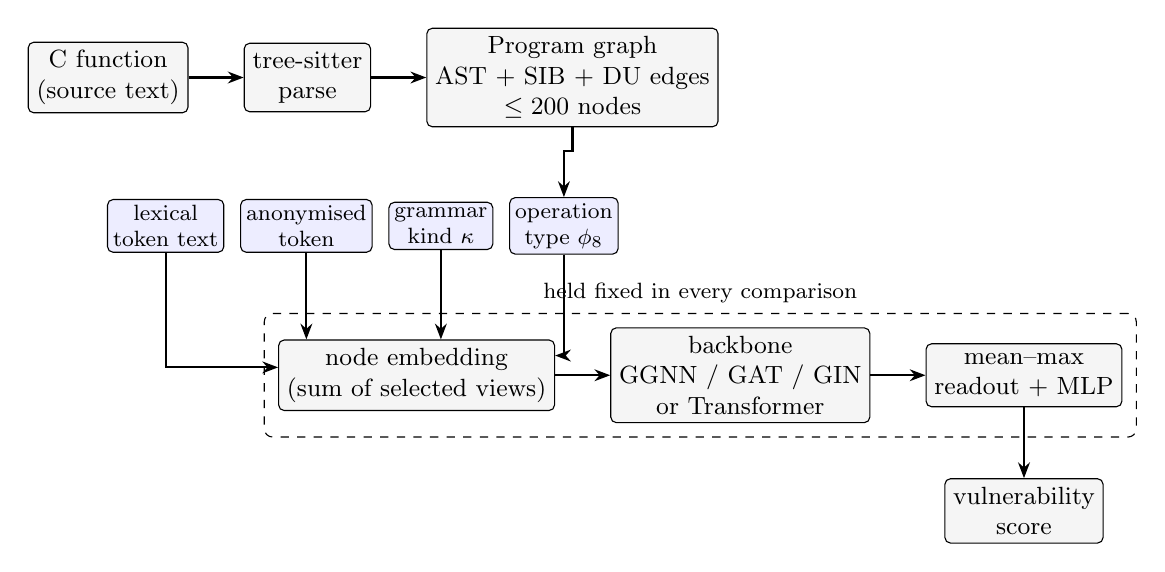
\begin{tikzpicture}[
  font=\small,
  box/.style={draw, rounded corners=2pt, minimum height=8mm, align=center,
              inner sep=3pt, fill=gray!8},
  view/.style={draw, rounded corners=2pt, minimum height=6mm, align=center,
               inner sep=2pt, fill=blue!7, font=\footnotesize},
  fixed/.style={draw, dashed, rounded corners=3pt, inner sep=5pt},
  arr/.style={-{Stealth[length=2mm]}, thick}]
  \node[box] (src) {C function\\(source text)};
  \node[box, right=7mm of src] (parse) {tree-sitter\\parse};
  \node[box, right=7mm of parse] (graph) {Program graph\\AST + SIB + DU edges\\$\le 200$ nodes};
  \node[view, below=11mm of parse, xshift=-18mm] (lex) {lexical\\token text};
  \node[view, right=2mm of lex] (anon) {anonymised\\token};
  \node[view, right=2mm of anon] (kind) {grammar\\kind $\kappa$};
  \node[view, right=2mm of kind] (op) {operation\\type $\phi_8$};
  \node[box, below=11mm of anon, xshift=14mm] (emb) {node embedding\\(sum of selected views)};
  \node[box, right=7mm of emb] (gnn) {backbone\\GGNN / GAT / GIN\\or Transformer};
  \node[box, right=7mm of gnn] (head) {mean--max\\readout + MLP};
  \node[box, below=9mm of head] (out) {vulnerability\\score};
  \draw[arr] (src) -- (parse);
  \draw[arr] (parse) -- (graph);
  \draw[arr] (graph.south) -- ++(0,-3mm) -| (op.north);
  \draw[arr] (lex.south) |- ($(emb.west)+(0,1mm)$);
  \draw[arr] (anon.south) -- (anon.south |- emb.north);
  \draw[arr] (kind.south) -- (kind.south |- emb.north);
  \draw[arr] (op.south) |- ($(emb.east)+(0,2.5mm)$);
  \draw[arr] (emb) -- (gnn);
  \draw[arr] (gnn) -- (head);
  \draw[arr] (head) -- (out);
  \begin{pgfonlayer}{background}
    \node[fixed, fit=(emb)(gnn)(head), label={[font=\footnotesize]above:held fixed in every comparison}] {};
  \end{pgfonlayer}
\end{tikzpicture}
\caption{Pipeline. The only component that varies between compared systems is
the choice of node view(s) (blue). The dashed region (embedding width, backbone
depth, readout, optimiser, training budget) is identical across views.
Evaluation always holds out whole projects}
\label{fig:pipeline}
\end{figure}

\paragraph{Running example} Consider the function body
\texttt{n = len(buf); p = av\_malloc(n * 4); if (!p) return -1;}.
A node of its tree can be described in four ways. Its \emph{lexical token} is
the text written in the source (\texttt{av\_malloc}, \texttt{n}, \texttt{buf}):
this is a property of the project that wrote it. Its \emph{anonymised token}
keeps only which names recur (\texttt{FUN\_0}, \texttt{VAR\_0},
\texttt{VAR\_1}). Its \emph{grammar kind} $\kappa$ is the name of the grammar
rule that produced it (\texttt{call\_expression}, \texttt{identifier},
\texttt{binary\_expression}), which depends only on the C language. Its
\emph{operation type} $\phi$ is a hand-built label for what the node does to
memory or control flow (\texttt{av\_malloc(...)} is a \texttt{MEMORY\_ACCESS}
node, \texttt{!p} a \texttt{COMPARISON}). Terms used throughout the paper
follow these four definitions.

\subsection{Program Graphs}
\label{sec:graph_construction}

Each function is parsed with \texttt{tree-sitter}, an incremental,
error-tolerant parser that recovers a usable tree from non-preprocessed C.
That property matters here: vulnerability corpora ship isolated functions
without their headers, so a parser requiring a complete translation unit
cannot be used. From the resulting tree we build $G = (\mathcal{V},
\mathcal{E})$:

\begin{itemize}
    \item $\mathcal{V}$: named AST nodes in pre-order, capped at 200;
    \item $\mathcal{E}_{AST}$: parent--child edges, both directions;
    \item $\mathcal{E}_{SIB}$: consecutive named siblings, giving source order;
    \item $\mathcal{E}_{DU}$: a def-use approximation linking successive
          occurrences of the same identifier leaf.
\end{itemize}

with $\mathcal{E} = \mathcal{E}_{AST} \cup \mathcal{E}_{SIB} \cup
\mathcal{E}_{DU}$, giving on average \numbigvulNodes{} nodes and \numbigvulEdges{} edges per
function in BigVul (\numdiversevulNodes{} and \numdiversevulEdges{} in DiverseVul). We state plainly that this is a syntax graph with a data-dependence
approximation, not a Code Property Graph~\citep{yamaguchi2014modeling}:
interprocedural control flow and points-to-precise dependence are absent.
Section~\ref{sec:limitations} discusses what that bounds.

\subsection{The Labelling Function $\phi$}
\label{sec:phi}

Let $K$ be the node-kind alphabet of the tree-sitter C grammar ($|K| = 363$)
and $\mathcal{T}_{32}$ the operation alphabet of Table~\ref{tab:taxonomy}. The
abstraction is a total function
\begin{equation}
    \phi : \mathcal{V} \longrightarrow \mathcal{T}_{32} \cup \{\bot\},
\label{eq:phi}
\end{equation}
where $\bot$ (\texttt{UNKNOWN}) labels nodes carrying no operation semantics.
$\phi$ is deterministic and needs no name resolution, no build system and no
whole-program context. It is defined by cases on the node's grammar kind:

\begin{enumerate}
    \item \textbf{Call expressions} are labelled by their callee name through
          $\psi$ (Section~\ref{sec:psi}); an unrecognised callee yields
          \texttt{CALL\_SITE}. User-defined functions, macros and calls
          through function pointers therefore all receive a label without
          resolution.
    \item \textbf{Kind-determined nodes} follow a fixed table:
          \texttt{subscript\_expression} $\to$ \texttt{ARRAY\_INDEX};
          \texttt{field\_expression} $\to$ \texttt{FIELD\_ACCESS};
          \texttt{cast\_expression} $\to$ \texttt{CAST};
          \texttt{if}/\texttt{switch}/\texttt{case} $\to$ \texttt{BRANCH\_*};
          loops $\to$ \texttt{LOOP\_*};
          \texttt{break}/\texttt{continue}/\texttt{goto}/\texttt{return} $\to$
          \texttt{JUMP\_*}/\texttt{RETURN};
          \texttt{assignment\_expression} and initialising declarators $\to$
          \texttt{ASSIGN}; \texttt{update\_expression} $\to$
          \texttt{ARITH\_ADD}.
    \item \textbf{Operator-determined nodes}: a \texttt{binary\_expression} is
          labelled by its operator token ($+\,-\ \to$ \texttt{ARITH\_ADD};
          $*\,/\ \to$ \texttt{ARITH\_MUL}; \texttt{\%} $\to$
          \texttt{ARITH\_MOD}; bitwise $\to$ \texttt{BITWISE\_OP}; shifts
          $\to$ \texttt{SHIFT\_OP}; equality $\to$ \texttt{COMPARISON\_EQ};
          relational $\to$ \texttt{COMPARISON\_REL}; logical $\to$
          \texttt{LOGICAL\_OP}). A \texttt{pointer\_expression} is
          \texttt{PTR\_DEREF} or \texttt{ADDR\_OF} by its prefix operator;
          unary \texttt{!} is \texttt{LOGICAL\_OP}.
    \item \textbf{Otherwise} $\phi(v) = \bot$.
\end{enumerate}

\subsubsection{Callee classification $\psi$}
\label{sec:psi}

$\psi$ maps a callee name to an operation class in two stages.

\textbf{Stage 1 (exact).} A fixed allow-list of C standard-library names,
grouped by the memory effect they carry: allocation, reallocation, release,
block copy, block set, string copy, concatenation, buffer-writing formatting,
length query, and stream I/O.

\textbf{Stage 2 (component).} Production C rarely calls those directly:
FFmpeg wraps allocation as \texttt{av\_malloc}, GLib as \texttt{g\_malloc},
the Linux kernel as \texttt{kmalloc}, OpenSSL as \texttt{OPENSSL\_malloc}.
Stage 2 splits the callee identifier into components on underscore and
camel-case boundaries and fires when a \emph{whole component} matches an
operation word.

Whole-component matching, rather than substring matching, is load-bearing.
Substring matching --- the obvious implementation --- is measurably wrong on
real code: it labels \texttt{\_\_put\_user} and \texttt{skb\_put} (writes) as
release operations via ``put'', \texttt{gen\_new\_label} as allocation via
``new'', \texttt{float64\_is\_zero} (a predicate) as a block set via ``zero'',
and \texttt{reallocate\_view} as reallocation, while \emph{missing}
\texttt{copy\_to\_user}, a genuine bounded copy.
Section~\ref{sec:rq_analysis} quantifies the resulting error.

We further separate stream I/O from buffer formatting. \texttt{printf} and
\texttt{fprintf} write to a stream and carry no caller-buffer overflow
semantics; only the \texttt{s*printf} and \texttt{scanf} families fill a
caller-supplied buffer. The distinction is not cosmetic: in our Devign sample
\texttt{fprintf} and \texttt{printf} alone account for 655 call sites, every
one of which a conflated rule would count as a memory operation.

\subsection{The Projection Lattice}
\label{sec:lattice}

Three granularities are defined --- $\mathcal{T}_{32}$ (finest),
$\mathcal{T}_{16}$, $\mathcal{T}_{8}$ --- related by surjections
\begin{equation}
    \pi_{16} : \mathcal{T}_{32} \to \mathcal{T}_{16}, \qquad
    \pi_{8}  : \mathcal{T}_{16} \to \mathcal{T}_{8},
\label{eq:projections}
\end{equation}
each extended to fix $\bot$. Coarser labellings are compositions,
$\phi_{16} = \pi_{16} \circ \phi$ and
$\phi_{8} = \pi_8 \circ \pi_{16} \circ \phi$, so the granularities are nested
\emph{by construction} rather than separately specified.

\begin{proposition}[Nesting]
\label{prop:nesting}
For all $u, v \in \mathcal{V}$, $\phi(u) = \phi(v) \Rightarrow \phi_{16}(u) =
\phi_{16}(v) \Rightarrow \phi_{8}(u) = \phi_{8}(v)$. Equivalently, the
partition of $\mathcal{V}$ induced by $\phi_8$ is coarser than that induced by
$\phi_{16}$, which is coarser than that induced by $\phi$.
\end{proposition}

\begin{proof}
Immediate from Eq.~\eqref{eq:projections}: $\phi_{16}$ and $\phi_8$ are
compositions of $\phi$ with total functions, and applying a function to equal
arguments yields equal results. The induced partitions are the preimages of a
chain of surjections, hence a chain of coarsenings.
\end{proof}

The consequence is that varying granularity varies exactly one quantity --- the
coarseness of a single labelling --- so the granularity experiment in
Section~\ref{sec:experiment} is interpretable, which a comparison of three
independently designed schemes would not be.

\begin{tableorg}[t]
\centering
\caption{The $|\mathcal{T}_8| = 8$ operation alphabet and the
$\mathcal{T}_{32}$ classes each abstracts. $\bot$ (\texttt{UNKNOWN}) labels
nodes with no operation semantics: declarations, identifiers, literals,
punctuation.}
\label{tab:taxonomy}
\adjustbox{max width=\textwidth}{%
\begin{tabular}{lll}
\toprule
$\mathcal{T}_8$ & abstracts ($\mathcal{T}_{32}$) & carries \\
\midrule
\texttt{MEMORY\_ACCESS} & \texttt{MEMORY\_\{ALLOC,REALLOC,FREE,COPY,SET\}}, \texttt{STRING\_\{COPY,CONCAT,FORMAT,LENGTH\}} & buffer lifetime, bounds \\
\texttt{ARRAY\_INDEX}   & \texttt{ARRAY\_INDEX} & indexed access \\
\texttt{PTR\_DEREF}     & \texttt{PTR\_DEREF}, \texttt{ADDR\_OF}, \texttt{FIELD\_ACCESS}, \texttt{CAST} & indirection \\
\texttt{CONTROL\_BRANCH}& \texttt{BRANCH\_\{IF,SWITCH\}}, \texttt{LOOP\_\{FOR,WHILE\}}, \texttt{JUMP\_\{BREAK,GOTO\}}, \texttt{RETURN} & reachability \\
\texttt{ARITH\_OP}      & \texttt{ARITH\_\{ADD,MUL,MOD\}}, \texttt{BITWISE\_OP}, \texttt{SHIFT\_OP} & value computation \\
\texttt{COMPARISON}     & \texttt{COMPARISON\_\{EQ,REL\}}, \texttt{LOGICAL\_OP} & guards \\
\texttt{CALL\_SITE}     & \texttt{CALL\_SITE}, \texttt{IO\_CALL} & unresolved or non-memory calls \\
\texttt{ASSIGN}         & \texttt{ASSIGN} & value flow \\
\bottomrule
\end{tabular}}
\end{tableorg}

\subsection{Node Views}
\label{sec:features}

A \emph{view} is the symbol (or symbols) from which a node's learned embedding
is looked up. Table~\ref{tab:modes} defines every view used in the paper. The
definitions matter for fairness, because a lexical baseline that carries no
information about node types would be compared against views that do. We
therefore also include the combinations that real detectors use: Devign and
ReVeal initialise a node with its code text together with its node
type~\citep{zhou2019devign, chakraborty2022deep}, which corresponds to our
\texttt{lex+$\kappa$} view.

\begin{tableorg}[t]
\centering
\caption{Node views. Leaves are tokens such as identifiers, literals and
keywords; internal nodes are the syntactic constructs above them. ``Invariant''
means the symbol alphabet is the same for every project. Embeddings of
combined views are summed.}
\label{tab:modes}
\adjustbox{max width=\textwidth}{%
\begin{tabular}{llllc}
\toprule
View & Leaf node carries & Internal node carries & Alphabet & Invariant \\
\midrule
\texttt{lexical} & source text ($\le 30$ chars, else \texttt{<LONG>}) & single token \texttt{<INTERNAL>} & training-fold tokens, at most 9{,}999 + \texttt{<UNK>} & no \\
\texttt{anon} & identifiers renamed by order of first appearance in the function, separately for variables, callees, fields, types and labels (\texttt{VAR\_i}, \texttt{FUN\_i}, \texttt{FIELD\_i}, \texttt{TYPE\_i}, \texttt{LABEL\_i}; index capped at 15); numbers $\to$ \texttt{NUM}; strings and characters $\to$ \texttt{STR}; free-text leaves such as comments by their node kind; other named leaves (e.g.\ primitive type names) keep their text & \texttt{<INTERNAL>} & $\approx$ 1{,}000 symbols & mostly \\
$\kappa$ & grammar kind & grammar kind & $|K|{+}1 = 364$ & yes \\
$\phi_8$ & operation type ($\bot$ if none) & operation type ($\bot$ if none) & 9 & yes \\
$\kappa{+}\phi$ & $\kappa$ and $\phi_8$ & $\kappa$ and $\phi_8$ & 364 and 9 & yes \\
\texttt{lex+$\kappa$} & lexical and $\kappa$ & \texttt{<INTERNAL>} and $\kappa$ & as above & no \\
\texttt{anon+$\kappa$} & anonymised and $\kappa$ & \texttt{<INTERNAL>} and $\kappa$ & as above & mostly \\
\bottomrule
\end{tabular}}
\end{tableorg}

\paragraph{The lexical view, precisely} Each leaf carries its exact source
text. Every internal node carries the same token \texttt{<INTERNAL>}, so the
plain lexical view contains \emph{no} node-type information; it is the
``text only'' condition. Tokens enter a per-fold dictionary built \emph{only}
from the training projects (the at most 9{,}999 most frequent tokens occurring at
least twice, plus \texttt{<UNK>}); every token not in that dictionary, including every token that
exists only in held-out projects, is mapped to a single \texttt{<UNK>}
embedding at test time. Out-of-vocabulary behaviour on unseen projects is
therefore part of what the lexical view is measured on.

\paragraph{Why anonymisation is a separate baseline} Anonymising identifiers
is the standard way to remove project vocabulary while keeping text
(Section~\ref{sec:background}). The \texttt{anon} and \texttt{anon+$\kappa$}
views isolate what grammar kinds add beyond that: if renaming identifiers
already closes the gap, the grammar kind is not needed.

\paragraph{The operation view} Our default combined view is
\begin{equation}
    \mathbf{x}_v = E_{\mathrm{op}}\big[\phi_8(v)\big]
                 + E_{\mathrm{kind}}\big[\kappa(v)\big],
\label{eq:features}
\end{equation}
where $E_{\mathrm{op}},E_{\mathrm{kind}}$ are learned tables with $9$ and $364$
rows. Both alphabets are fixed by the C grammar and the taxonomy, hence
identical across projects and corpora.

One caveat, stated precisely. Node \emph{features} contain no identifier, but
$\phi$ \emph{consults} identifier text to classify a callee, so a bounded
amount of name-derived information (at most
$\log_2(|\mathcal{T}_{32}|+1) \approx 5$ bits per call node) influences the
representation. What does not survive is the identifier itself, its spelling,
or any project-specific vocabulary.

\subsection{Networks and training, in brief}
\label{sec:networks}

A \emph{backbone} is the network that passes information between nodes. We use
three message-passing networks over the program graph: a gated graph neural
network (\textbf{GGNN}), in which each node updates its state from its
neighbours with a gated recurrent unit; a graph attention network
(\textbf{GAT}), which weights neighbours by learned attention; and a graph
isomorphism network (\textbf{GIN}), which sums neighbour states and passes them
through a small perceptron. A fourth, non-graph backbone is a \textbf{Transformer}
encoder that applies self-attention over the nodes listed in \emph{pre-order}
(the order in which a depth-first walk first visits them) and ignores the
edges. After the backbone, a \emph{readout} pools the node vectors into one
vector per function (the concatenation of their element-wise mean and
maximum), and a small perceptron outputs the vulnerability score. Training
minimises a binary cross-entropy in which vulnerable functions are weighted up
by the benign-to-vulnerable ratio of the training set (capped at 20)
\emph{(class-weighted loss)}. ``Def-use'' edges connect successive occurrences
of the same identifier, a cheap stand-in for data flow; ``named nodes'' are the
syntax-tree nodes the grammar names (punctuation tokens are excluded).

\subsection{Algorithms}
\label{sec:algorithms}

Algorithm~\ref{alg:graph} gives the construction of a node's views;
Algorithm~\ref{alg:protocol} gives the evaluation protocol that every reported
number follows.

\begin{algorithm}[t]
\caption{Program graph and node views for one function}
\label{alg:graph}
\begin{algorithmic}[1]
\Require C source $f$, node cap $N=200$
\State $T \leftarrow \textsc{TreeSitterParse}(f)$
\State $V \leftarrow$ first $N$ named nodes of $T$ in pre-order; record $n_{\text{full}}=|\text{named nodes}|$
\For{each $v \in V$}
  \State $\kappa(v) \leftarrow$ grammar kind of $v$
  \State $\phi(v) \leftarrow$ \textbf{case} kind of $v$:
  \State \quad call: $\psi(\text{callee name})$ \Comment{exact allow-list, then whole-component match}
  \State \quad kind-determined: table lookup \Comment{rule 2 of Section~\ref{sec:phi}}
  \State \quad binary / pointer / unary: by operator token
  \State \quad otherwise $\bot$
  \If{$v$ is a leaf}
     \State $\text{lex}(v) \leftarrow$ source text of $v$;\ $\text{anon}(v) \leftarrow \textsc{Rename}(v)$ \Comment{first occurrence in $f$}
  \Else
     \State $\text{lex}(v) \leftarrow \text{anon}(v) \leftarrow \texttt{<INTERNAL>}$
  \EndIf
\EndFor
\State $\mathcal{E} \leftarrow$ AST edges (both directions) $\cup$ sibling edges $\cup$ def-use edges between successive occurrences of an identifier
\State \Return graph $(V,\mathcal{E})$ with views $\kappa,\phi,\text{lex},\text{anon}$ per node
\end{algorithmic}
\end{algorithm}

\begin{algorithm}[t]
\caption{Cross-project evaluation of one (view, backbone) system}
\label{alg:protocol}
\begin{algorithmic}[1]
\Require corpus sample $D$ (uniform random, seeded), view $m$, backbone $b$
\State remove near-duplicates from $D$ by their $(\kappa,\phi)$ node sequences
\State hold the projects whose size exceeds $0.3\times$ the mean fold train-only
\State deal the other projects into $5$ folds, twice with different shuffles: $10$ folds
\For{fold $k=1,\dots,10$}
   \State train set $\leftarrow$ all functions of projects not in fold $k$
   \State fit the lexical dictionary on the train set only
   \State initialise model with seed $1000+k$; train for $10$ epochs with class-weighted loss
   \State score the held-out projects; store AUC, AUPRC and the raw scores
\EndFor
\State compare two systems by paired fold differences (Wilcoxon) and a cluster bootstrap over held-out projects
\end{algorithmic}
\end{algorithm}


\section{Experimental Design}
\label{sec:experiment}

\subsection{Research questions}
\begin{itemize}
    \item \textbf{RQ1 (the labelling function as an analysis).} How accurately
          does $\phi$ identify memory and string operations, measured against
          independent blind annotation on the corpora used in the
          experiments?
    \item \textbf{RQ2 (which node view transfers).} With the graph, backbone
          and training budget fixed, how does cross-project detection change
          when the node view changes? In particular: does the grammar kind
          $\kappa$ beat text; does it beat text \emph{plus} node type; does it
          beat anonymised text; and does the engineered taxonomy $\phi$ add
          anything to $\kappa$?
    \item \textbf{RQ3 (generality).} Does the effect hold across two corpora
          and across four architectures, including a Transformer?
    \item \textbf{RQ4 (ablations).} Which parts of the graph and of the
          taxonomy matter?
    \item \textbf{RQ5 (reference points).} How do the results compare with
          re-implementations of existing input representations, with a
          pretrained code model, and with a trivial function-size rule?
\end{itemize}

\subsection{Corpora, sampling and class balance}
\label{sec:corpora}

We use BigVul~\citep{fan2020bigvul} and DiverseVul~\citep{chen2023diversevul},
loaded from pinned public mirrors, plus Devign~\citep{zhou2019devign} for the
analysis validation only. From each of BigVul and DiverseVul we draw
\numcfgN{} functions \emph{uniformly at random} without replacement (a fixed
seed, so the sample is reproducible), after which near-duplicates are removed
(Section~\ref{sec:dedup}). This replaces an earlier design that took the first
rows in corpus order; it also raises the number of vulnerable functions from
about 430 to \numbigvulVuln{} (BigVul) and \numdiversevulVuln{} (DiverseVul).
Table~\ref{tab:corpora} gives the resulting properties.


\begin{tableorg}[t]
\centering
\caption{Corpus properties measured on our uniform random samples
(10{,}000 functions drawn per corpus, then de-duplicated). \emph{Prevalence} is
the fraction of vulnerable functions in the whole sample; \emph{Test prev.} is
the pooled fraction over the held-out folds. They differ because the largest
repositories, which have a lower share of vulnerable functions, are held
train-only and never appear in a test fold (Section~\ref{sec:protocol}).
\emph{Truncated} is the percentage of functions with more than 200 named AST
nodes, overall / vulnerable / benign.}
\label{tab:corpora}
\adjustbox{max width=\textwidth}{%
\begin{tabular}{lrrrrrrrr}
\toprule
Corpus & Functions & Vulnerable & Prevalence & Test prev. & Projects & Top-2 share & Nodes (mean) & Truncated (\%) \\
\midrule
BigVul & 9,435 & 555 & 0.059 & 0.071 & 250 & 64.3\% & 96 & 18.1 / 42.3 / 16.6 \\
DiverseVul & 9,791 & 567 & 0.058 & 0.059 & 633 & 25.0\% & 110 & 25.6 / 53.4 / 23.9 \\
Devign & 9,666 & 4,455 & 0.461 & --- & 2 & 100.0\% & 137 & 41.2 / 44.3 / 38.6 \\
\bottomrule
\end{tabular}}
\end{tableorg}

Table~\ref{tab:node_dist} gives the distribution of operation types over
the nodes of the BigVul sample: about three quarters of nodes carry no
operation label ($\bot$) but keep their grammar kind, and memory operations are
rare.


\begin{tableorg}[t]
\centering
\caption{Node-type distribution under $\phi_8$ (BigVul sample). $\bot$
(\texttt{UNKNOWN}) nodes carry no operation label but keep their grammar kind.}
\label{tab:node_dist}
\begin{tabular}{lr@{\hskip 2em}lr}
\toprule
Type & Share & Type & Share \\
\midrule
$\bot$ (\texttt{UNKNOWN}) & 75.23\% & \texttt{COMPARISON} & 2.72\% \\
\texttt{PTR\_DEREF} & 6.56\% & \texttt{ARITH\_OP} & 1.57\% \\
\texttt{CALL\_SITE} & 5.45\% & \texttt{ARRAY\_INDEX} & 0.53\% \\
\texttt{CONTROL\_BRANCH} & 4.18\% & \texttt{MEMORY\_ACCESS} & 0.30\% \\
\texttt{ASSIGN} & 3.47\% &  &  \\
\bottomrule
\end{tabular}
\end{tableorg}

\paragraph{The data are strongly imbalanced, and we do not rebalance them}
Only \numbigvulPrev{} of BigVul and \numdiversevulPrev{} of DiverseVul
functions are labelled vulnerable. We handle this in three ways. (i)~Training
uses a class-weighted loss, with positive weight equal to the training
benign-to-vulnerable ratio capped at 20. (ii)~Test sets are never resampled, so
every metric reflects the true prevalence. (iii)~We report AUC and AUPRC, which
do not depend on a decision threshold, together with the trivial
``everything is vulnerable'' classifier as a floor; its $F_1$ at the observed
test prevalence is only $2p/(1{+}p)$.

\paragraph{Why overall prevalence and test prevalence differ} In BigVul the
overall prevalence is \numbigvulPrev{} but the pooled prevalence of the
held-out folds is \numbigvulTestPrev{}. The reason is the train-only rule of
Section~\ref{sec:protocol}: the largest repositories (Chrome and the Linux
kernel; \numbigvulTrainOnlyN{} functions, prevalence \numbigvulTrainOnlyPrev{})
are never tested, and the remaining projects have a higher vulnerable share. An
earlier version of this paper quoted these two figures (0.054 and 8.8\%) without
connecting them.

\paragraph{Project concentration} Even after the largest repositories are held
train-only, one project can dominate a test fold: in BigVul the repository
\texttt{\numbigvulTopTestProject} makes up as much as
\numbigvulTopTestShareMax\% of a fold's test functions (the largest share in any
DiverseVul fold is \numdiversevulTopTestShareMax\%). We therefore report every
main BigVul comparison a second time with that project removed from the test
predictions (Section~\ref{sec:rq_representation}).

\paragraph{The 200-node cap} A graph keeps the first 200 named nodes in
pre-order. Table~\ref{tab:corpora} shows that this truncates
\numbigvulTruncPct\% of BigVul functions and \numdiversevulTruncPct\% of
DiverseVul functions, and that it is far from class-neutral: in BigVul
\numbigvulTruncVulnPct\% of vulnerable functions are truncated against
\numbigvulTruncBenignPct\% of benign ones (Fisher exact test
$p$~\numbigvulTruncP). Vulnerable functions are simply longer. This matters in
two ways, both examined below: a model may learn function length rather than
anything about vulnerabilities (Section~\ref{sec:rq_reference}), and what lies
beyond the cap is invisible to every compared system alike.

\subsection{Deduplication}
\label{sec:dedup}
Near-duplicate functions are removed \emph{before} any split. Vendored code
appears under several project names, so without this step a held-out function
can have a twin in training. Signatures are computed over the abstracted node
sequences ($\kappa$ and $\phi$), which catches renamed copies that text hashing
misses (the signature also includes the node count, which is capped at 200,
so long functions that agree on their first 200 nodes are treated as copies;
the first occurrence is kept whichever label it carries); this removes 2--6\% of the sampled functions (the remaining counts are
in Table~\ref{tab:corpora}).

\subsection{Cross-project protocol}
\label{sec:protocol}
Evaluation uses project-level GroupKFold with ten folds in every experiment:
projects are dealt into five folds twice, with two different shuffles, and no
project is ever split between training and test. Projects too large to be placed
without dominating a fold (those larger than 30\% of the mean fold size: Chrome and the Linux kernel in
BigVul, the Linux kernel only in DiverseVul) are held \emph{train-only}. Every
condition in every table is run on the same ten folds; the analysis scripts
refuse to merge result files whose fold assignments differ. The two repeats are
\emph{not} independent: the splitter deals the projects out largest first, so
the largest held-out projects fall into the same fold index in both repeats
(for example the repository that dominates BigVul test folds appears in folds 0
and 5), while the small projects are reshuffled (the test project sets of fold
$k$ and $k+5$ overlap by only 13--23\% in Jaccard index). The ten folds are
therefore better described as five folds with partial replication.
Section~\ref{sec:stats} says how the tests account for this.

\paragraph{Per-fold training} The lexical dictionary is built from the training
projects only (Section~\ref{sec:features}); the classifier is initialised and
shuffled with seed $1000+k$ on fold $k$, the same seed for every compared
system. Hyper-parameters are in Table~\ref{tab:hparams}. They were fixed before
the experiments and are not tuned on any fold; there is no validation split and
no early stopping, so every system trains for exactly \numcfgEpochs{} epochs.


\begin{tableorg}[t]
\centering
\caption{Hyper-parameters. All values are fixed in advance and shared by every
compared system; none is tuned on any fold.}
\label{tab:hparams}
\begin{tabular}{lp{0.62\linewidth}}
\toprule
Item & Value \\
\midrule
Embedding width / hidden width & 64 / 128 \\
Message-passing layers & 2 (GGNN: 2 gated steps) \\
Transformer & 2 layers, 4 heads, feed-forward $2\times$ width, dropout 0.1 \\
Readout and head & mean $\Vert$ max pooling; MLP $2h\to h/2\to 1$, dropout 0.3 \\
Optimiser & Adam, learning rate 0.001 \\
Batch size & 64 \\
Epochs & 10 (fixed; no early stopping, no validation split) \\
Loss & binary cross-entropy, positive weight $=\min(n_{\text{neg}}/n_{\text{pos}}, 20)$ \\
Seeds & initialisation and shuffling seed $1000+k$ for fold $k$, shared by all systems \\
Lexical dictionary & up to 9{,}999 most frequent training-fold tokens with count $\ge 2$, plus \texttt{<UNK>} \\
Node cap & 200 named AST nodes (pre-order) \\
Sample & 10,000 functions per corpus, uniform at random, seed 0 \\
Folds & 5$\times$2 = 10 project-level folds \\
Pretrained reference & UniXcoder-base, 256 tokens, frozen; logistic regression $C=0.1$, balanced \\
\bottomrule
\end{tabular}
\end{tableorg}

\subsection{Statistical treatment}
\label{sec:stats}
Every paired comparison is made between two systems on the folds both
completed. The reported difference is the \emph{mean over folds} of the
per-fold difference in the metric, which is the quantity the per-fold columns of
the tables average. We attach three kinds of uncertainty statement.
\begin{enumerate}
    \item A \textbf{cluster bootstrap over held-out projects}. In each of the
          resamples, projects are drawn with replacement (a project is one
          cluster however many folds it is tested in); every function of a drawn
          project is repeated as often as the project was drawn; the metric
          difference is recomputed inside each fold and averaged. The 95\%
          percentile interval and a two-sided $p$ follow. Functions inside a
          repository share style, APIs and often code, so resampling functions
          instead would understate the uncertainty. We use 1{,}000 resamples
          under each of five seeds for AUC (the verdict is called stable if the
          interval excludes zero under at least 90\% of the seeds), and 500
          resamples under one seed for AUPRC and the size-binned AUC.
    \item A \textbf{Wilcoxon signed-rank test}~\citep{wilcoxon1945individual}, a
          paired test that uses only the ranks of the ten per-fold differences
          (exact, two-sided; its smallest attainable $p$ is $0.002$). Because
          fold $k$ and fold $k+5$ are partial replicates of each other
          (Section~\ref{sec:protocol}), we also run it on the five
          repeat-averaged differences, where the smallest attainable $p$ is
          $0.0625$, so that test can never reach the 5\% level on its own.
    \item \textbf{Holm-adjusted $p$-values}~\citep{holm1979simple}, which
          correct a family of tests for the chance that one of them looks
          significant by luck. The family is all contrasts for one corpus and
          metric; adjusted values are stored in the result files and quoted where
          a conclusion depends on one contrast.
\end{enumerate}
We therefore treat the cluster bootstrap as the primary inference, the Wilcoxon
test as supporting evidence, and call a difference supported only if the
bootstrap interval excludes zero. Whether truncation depends on the label is a
question about counts, for which we use Fisher's exact test (a small-sample
alternative to the chi-square test of independence).

\subsection{Compute and reproducibility}
All experiments run on CPU. One run of the BigVul GGNN grid takes roughly
seven minutes per cell per core. Every table and every number in the text is
generated from the stored per-fold predictions by scripts in the repository
(\texttt{experiments/run\_all.sh}); no result is typed by hand.


\subsection{RQ1: $\phi$ as a static analysis}
\label{sec:rq_analysis}

\paragraph{Design} An abstraction that is evaluated only by what it does for a
downstream classifier can hide errors in its own labels. We therefore score
$\phi$'s callee classification against annotated ground truth. This version of
the validation differs from the one in the first submission of this work in
three respects, each responding to a concern that a validation of this kind is
only as good as its annotation.

\begin{itemize}
    \item \textbf{The experimental corpora.} Callee names and one
          example call each are drawn from the \emph{experimental samples} of
          BigVul and DiverseVul, not only from Devign; Devign (not used in the
          detection experiments) is kept so that the new labels can be compared
          with the first submission's. The sample is stratified
          over $\phi$'s predicted classes (up to 14 names per class, half from
          the most frequent names and half at random) plus 100 names drawn
          from callees that $\phi$ left unlabelled, so that recall is
          estimable. The Devign gold set of the original submission is
          annotated again.
    \item \textbf{Independent, blind annotation.} Each name is labelled by two
          annotators who see only the name, its frequency and one example call;
          they never see $\phi$'s prediction, each other's labels, or the
          analysis code. The criteria are written down in advance
          (\texttt{experiments/annotations/PROTOCOL.md}). The two annotators
          are language-model annotators of different capability, run as
          separate sessions. No human annotated these sheets.
    \item \textbf{Agreement and adjudication.} We report raw agreement and
          Cohen's $\kappa$~\citep{cohen1960coefficient} between the two annotators; every disagreement is
          resolved by a third blind pass that sees the two candidate labels in
          random order. The consensus is the ground truth for scoring. We also
          score against each annotator alone to show sensitivity.
\end{itemize}

\paragraph{Who annotated the original gold set} The 212 Devign labels of the
first submission were assigned by a single annotator from written criteria. The sheet
that annotator worked from listed $\phi$'s predicted class next to each name,
so the annotation was not blind to the analysis under test, and the labels are
stored in a script in which every name not listed defaults to ``none''. That
is a weaker protocol than the blind one above.
Their agreement with the new consensus is $\kappa_C=\numdevignOrigKappa$,
so the original labels were largely sound but are not used for the headline
scores here.

Tables~\ref{tab:rq1_analysis} and~\ref{tab:rq1_agreement} give the per-class
scores and the annotation agreement.


\begin{tableorg}[t]
\centering
\caption{RQ1: $\phi$ as a static analysis, scored against the consensus of two
blind annotators and a third pass on disagreements, pooled over the three
corpora. Brackets are 95\% Wilson intervals; tp/fp/fn are counts of distinct
callee names. The last row scores the question $\phi_8$ actually answers
(memory or string operation vs. not).}
\label{tab:rq1_analysis}
\begin{tabular}{lrrr}
\toprule
Class & Precision & Recall & tp/fp/fn \\
\midrule
\texttt{MEMORY\_ALLOC} & 0.88 $[0.75,0.94]$ & 0.78 $[0.65,0.87]$ & 42/6/12 \\
\texttt{MEMORY\_REALLOC} & 0.97 $[0.85,0.99]$ & 0.94 $[0.82,0.98]$ & 34/1/2 \\
\texttt{MEMORY\_FREE} & 0.85 $[0.73,0.93]$ & 0.95 $[0.85,0.99]$ & 41/7/2 \\
\texttt{MEMORY\_COPY} & 0.63 $[0.46,0.77]$ & 0.88 $[0.70,0.96]$ & 22/13/3 \\
\texttt{MEMORY\_SET} & 1.00 $[0.83,1.00]$ & 0.95 $[0.76,0.99]$ & 19/0/1 \\
\texttt{STRING\_COPY} & 1.00 $[0.90,1.00]$ & 0.82 $[0.68,0.91]$ & 33/0/7 \\
\texttt{STRING\_CONCAT} & 0.97 $[0.83,0.99]$ & 0.93 $[0.79,0.98]$ & 28/1/2 \\
\texttt{STRING\_FORMAT} & 0.86 $[0.71,0.94]$ & 0.88 $[0.73,0.95]$ & 30/5/4 \\
\texttt{STRING\_LENGTH} & 0.97 $[0.83,0.99]$ & 0.97 $[0.83,0.99]$ & 29/1/1 \\
\texttt{IO\_CALL} & 0.86 $[0.74,0.93]$ & 0.69 $[0.57,0.79]$ & 43/7/19 \\
\midrule
Macro & 0.90 & 0.88 & \\
Memory operation (any of the 9) & 0.94 & 0.94 & 293/19/19 \\
\bottomrule
\end{tabular}
\end{tableorg}

\begin{tableorg}[t]
\centering
\caption{RQ1: annotation agreement and per-corpus scores. Agreement and
Cohen's $\kappa_{C}$ are between the two blind annotators before adjudication;
precision and recall are macro-averaged over classes against the consensus; the
last column is precision / recall for ``memory or string operation''.}
\label{tab:rq1_agreement}
\adjustbox{max width=\textwidth}{%
\begin{tabular}{lrrrrrr}
\toprule
Corpus & Names & Agreement & $\kappa_{C}$ & Macro P & Macro R & Memory-op P / R \\
\midrule
Devign & 212 & 0.92 & 0.89 & 0.90 & 0.87 & 0.90 / 0.93 \\
BigVul & 227 & 0.94 & 0.93 & 0.90 & 0.87 & 0.95 / 0.95 \\
DiverseVul & 236 & 0.92 & 0.90 & 0.89 & 0.89 & 0.96 / 0.94 \\
\bottomrule
\end{tabular}}
\end{tableorg}

\paragraph{Agreement} Table~\ref{tab:rq1_agreement} reports agreement per corpus.
Before adjudication the two blind annotators agree on \numpooledAgree{} of the
\numpooledNNames{} names (pooled Cohen's kappa $\kappa_C=\numpooledKappa$; per
corpus, raw agreement and $\kappa_C$: Devign \numdevignAgree{} and
\numdevignKappa, BigVul \numbigvulAgree{} and \numbigvulKappa, DiverseVul
\numdiversevulAgree{} and \numdiversevulKappa), conventionally read as almost
perfect agreement. \numdevignAdjudicated, \numbigvulAdjudicated{} and
\numdiversevulAdjudicated{} disagreements respectively went to the third pass; in
\numdevignUnresolved{} Devign case(s) the third annotator agreed with neither of
the first two and its label was used.

\paragraph{Accuracy of $\phi$} Against the consensus, macro-averaged precision
is \numpooledMacroP{} and recall \numpooledMacroR{} over the ten callee classes
(Table~\ref{tab:rq1_analysis}); these are lower than the $0.976$ reported for
the original single-annotator labels, which we now regard as optimistic. The
weakest class is \texttt{MEMORY\_COPY}, with precision \numcopyPrecision{}. Two
caveats keep these figures honest. First, several classes have few positives
(the smallest has \numminClassPositives), so their intervals are wide;
Table~\ref{tab:rq1_analysis} shows Wilson intervals~\citep{wilson1927probable} rather than only the point
values. Second, the sample is stratified, so the numbers are per-name
estimates, not a population-weighted accuracy.

\paragraph{What $\phi_8$ actually needs} At $|\mathcal{T}|=8$ every memory and
string class collapses into a single \texttt{MEMORY\_ACCESS} type, so confusing
an allocation with a copy costs nothing. The question that matters is whether a
callee is a memory or string operation at all. On that question precision is
\numpooledMemopP{} and recall \numpooledMemopR{} pooled over the three corpora
(\numbigvulMemopP{}/\numbigvulMemopR{} on BigVul,
\numdiversevulMemopP{}/\numdiversevulMemopR{} on DiverseVul).

\paragraph{Residual disagreements} The informative ones are structural, not
noise. QEMU's \texttt{tcg\_temp\_free*} releases an intermediate-representation
temporary rather than heap memory, so a release rule fires on it. Wrappers that
allocate \emph{and} copy or format (\texttt{g\_strdup},
\texttt{g\_strdup\_printf}, \texttt{string\_sprintf}) cannot be given a single
class by a single-label taxonomy. Project-specific I/O and teardown helpers
(\texttt{bdrv\_pread}, \texttt{ReadBlobMSBLong}, \texttt{RelinquishMagickMemory})
are missed because they match no allow-list entry and no whole-identifier-
component rule. These are limitations of a name-based analysis with no type
information; they bound what $\phi$ can claim and are one reason we do not
expect it to beat the parser's own alphabet.

\paragraph{What the validation changed in the design} Matching whole identifier
components instead of substrings removes writes and predicates mislabelled as
releases and allocations (\texttt{\_\_put\_user}, \texttt{skb\_put},
\texttt{gen\_new\_label}, \texttt{float64\_is\_zero}); separating stream I/O
from buffer formatting keeps 655 \texttt{printf}/\texttt{fprintf} call sites in
one corpus out of the memory class; and restricting the copy rule to explicit
copy primitives raises its precision at the cost of recall. These three changes
predate the present evaluation and are unchanged.


\subsection{RQ2: which node view transfers across projects}
\label{sec:rq_representation}

\emph{In short:} on projects never seen in training, a network that reads
identifier text from scratch performs close to chance; removing the project
vocabulary (by renaming identifiers or by using grammar kinds) lifts AUC by
roughly \numdeltaMin{} to \numdeltaMax{}; and the choice among the vocabulary-free views matters
much less than the choice to leave the vocabulary out.

Everything except the node view is held fixed: graph, backbone (GGNN), depth,
width, readout, optimiser, class weighting and gradient budget.
Table~\ref{tab:rq2_representation} reports the BigVul results over 10 matched
folds, and Table~\ref{tab:direct} the direct paired contrasts between views.


\begin{tableorg}[t]
\centering
\caption{RQ2: node views on BigVul, GGNN, 10 matched project-level folds
(mean $\pm$ population std over folds). Differences are paired against the
lexical baseline: each $\Delta$ cell reads mean per-fold difference, 95\%
cluster-bootstrap interval over held-out projects, bootstrap $p$ / Wilcoxon
signed-rank $p$ over folds; \emph{n.s.} marks an interval containing zero.
\emph{AUC in size bins} is the AUC computed within five bins of function size
(0.5 = no information beyond length). AUPRC is reported without paired tests.}
\label{tab:rq2_representation}
\adjustbox{max width=\textwidth}{%
\begin{tabular}{lrrlrr}
\toprule
Node view & Folds & AUC & $\Delta$AUC [95\% CI] $p_{\text{boot}}$ / $p_{\text{W}}$ & AUC in size bins & AUPRC \\
\midrule
Trivial (all-positive) & --- & 0.500 & --- & 0.500 & 0.071 \\
Function size only (rule) & 10 & 0.736 $\pm$ 0.065 & --- & 0.500 & 0.232 $\pm$ 0.087 \\
Lexical token & 10 & 0.506 $\pm$ 0.077 & --- & 0.467 & 0.085 $\pm$ 0.034 \\
Anonymised token & 10 & 0.708 $\pm$ 0.046 & $+0.202$ $[+0.149, +0.249]$ $<0.001$ / 0.002 & 0.569 & 0.167 $\pm$ 0.048 \\
Operation type $\phi_8$ & 10 & 0.649 $\pm$ 0.052 & $+0.143$ $[+0.092, +0.211]$ $<0.001$ / 0.010 & 0.497 & 0.117 $\pm$ 0.026 \\
Grammar kind $\kappa$ & 10 & 0.691 $\pm$ 0.037 & $+0.185$ $[+0.130, +0.236]$ $<0.001$ / 0.002 & 0.535 & 0.149 $\pm$ 0.027 \\
Operation $+$ kind ($\kappa{+}\phi$) & 10 & 0.687 $\pm$ 0.060 & $+0.181$ $[+0.132, +0.236]$ $<0.001$ / 0.002 & 0.536 & 0.158 $\pm$ 0.042 \\
Lexical $+$ kind & 10 & 0.592 $\pm$ 0.072 & $+0.086$ $[+0.038, +0.111]$ $<0.001$ / 0.002 & 0.519 & 0.105 $\pm$ 0.039 \\
Anonymised $+$ kind & 10 & 0.701 $\pm$ 0.059 & $+0.195$ $[+0.144, +0.244]$ $<0.001$ / 0.002 & 0.558 & 0.180 $\pm$ 0.059 \\
\bottomrule
\end{tabular}}
\end{tableorg}


\begin{tableorg}[t]
\centering
\caption{Direct paired contrasts between node views (GGNN, 10 matched folds):
$\Delta$AUC of the first view minus the second, with 95\% cluster-bootstrap
interval, bootstrap $p$ / Wilcoxon $p$. These are the comparisons a reader
needs to judge whether one view is better than another; a difference between
two views' gaps to the lexical baseline is not a test of the difference.}
\label{tab:direct}
\adjustbox{max width=\textwidth}{%
\begin{tabular}{lll}
\toprule
Contrast & BigVul & DiverseVul \\
\midrule
$\kappa{+}\phi$ vs $\kappa$ & $-0.004$ $[-0.017, +0.021]$ 0.920\,n.s. / 1.000 & $+0.008$ $[-0.005, +0.022]$ 0.232\,n.s. / 0.027 \\
$\kappa$ vs lexical$+\kappa$ & $+0.100$ $[+0.064, +0.156]$ $<0.001$ / 0.002 & $+0.060$ $[+0.030, +0.088]$ $<0.001$ / 0.002 \\
$\kappa$ vs anonymised$+\kappa$ & $-0.010$ $[-0.038, +0.014]$ 0.380\,n.s. / 0.625 & $-0.012$ $[-0.030, +0.002]$ 0.098\,n.s. / 0.322 \\
anonymised$+\kappa$ vs lexical$+\kappa$ & $+0.110$ $[+0.079, +0.166]$ $<0.001$ / 0.002 & $+0.071$ $[+0.043, +0.102]$ $<0.001$ / 0.004 \\
lexical$+\kappa$ vs lexical & $+0.086$ $[+0.038, +0.111]$ $<0.001$ / 0.002 & $+0.042$ $[+0.021, +0.061]$ $<0.001$ / 0.037 \\
anonymised vs lexical & $+0.202$ $[+0.149, +0.249]$ $<0.001$ / 0.002 & --- \\
$\kappa$ vs $\phi_8$ & $+0.042$ $[-0.004, +0.067]$ 0.072\,n.s. / 0.049 & --- \\
9-dim bottleneck $\kappa$ vs $\kappa$ & $+0.017$ $[+0.004, +0.040]$ 0.018 / 0.322 & --- \\
\bottomrule
\end{tabular}}
\end{tableorg}

\paragraph{Text read from scratch does not transfer} With the lexical view
the GGNN reaches AUC \mBvGgnnLexAuc{} on BigVul and \mDvGgnnLexAuc{} on
DiverseVul, close to the $0.5$ of a random ranking (across all lexical cells, \numlexAucMin{} to \numlexAucMax{}). The cause is visible in the
mechanism: after the per-fold cut, tokens that occur only in held-out projects
map to \texttt{<UNK>}, and what remains of the vocabulary correlates with
project identity rather than with the weakness.

\paragraph{Vocabulary-free views transfer} Replacing text with the grammar kind
raises AUC by \cBvGgnnKindVLexD{} (95\% CI \cBvGgnnKindVLexLo{} to
\cBvGgnnKindVLexHi{}; bootstrap $p$ \cBvGgnnKindVLexP{}; Wilcoxon $p$
\cBvGgnnKindVLexW{}; \cBvGgnnKindVLexWins{} folds won) on BigVul, and by
\cDvGgnnKindVLexD{} (\cDvGgnnKindVLexLo{} to \cDvGgnnKindVLexHi{}) on
DiverseVul. Renaming identifiers while keeping all other token text
(\emph{anonymised}) gives \cBvGgnnAnonVLexD{}
(\cBvGgnnAnonVLexLo{} to \cBvGgnnAnonVLexHi{}) on BigVul. The effect is large
relative to the fold-to-fold spread of the lexical view
(standard deviation \numbvGgnnLexicalAucStd{} AUC; Table~\ref{tab:rq2_representation}).
After Holm adjustment over the whole family of contrasts on BigVul the
bootstrap $p$ of the $\kappa$-versus-text contrast remains
\cBvGgnnKindVLexH{}; the fold-level Wilcoxon test, whose smallest possible $p$
is $0.002$ before adjustment, reaches \cBvGgnnKindVLexWH{} after it, and
\cBvGgnnKindVLexWblk{} on the five repeat-averaged differences, so that test
alone cannot carry the claim; the cluster bootstrap does.

\paragraph{The grammar kind is not better than anonymised text} This is the
conclusion that changed most since the first version of this work. Reviewing it
we added the baselines that a text-only comparison omits: anonymised tokens, and
each of text and anonymised tokens combined with the kind
(Section~\ref{sec:features}). The direct contrast of $\kappa$ against
anonymised$+\kappa$ is \cBvGgnnKindVAnonKindD{}
(\cBvGgnnKindVAnonKindLo{} to \cBvGgnnKindVAnonKindHi{}) on BigVul and
\cDvGgnnKindVAnonKindD{} (\cDvGgnnKindVAnonKindLo{} to
\cDvGgnnKindVAnonKindHi{}) on DiverseVul
(Table~\ref{tab:direct}). The same contrast against anonymised text alone (run on BigVul only) is
\cBvGgnnKindVAnonD{} (\cBvGgnnKindVAnonLo{} to \cBvGgnnKindVAnonHi{}). All
intervals include zero. Identifier renaming, which is what sequence-based
detectors have long done as preprocessing, therefore recovers essentially the
whole benefit, to within the precision of this study. What the grammar kind offers is the same effect without any
preprocessing choice, not a better effect.

\paragraph{Adding node type to text helps, but less than removing the text}
The Devign-style combination of text with the node type improves on text alone
by \cBvGgnnLexKindVLexD{} (\cBvGgnnLexKindVLexLo{} to
\cBvGgnnLexKindVLexHi{}) on BigVul, so part of the benefit of structure is
independent of removing names. But $\kappa$ alone beats that combination by
\cBvGgnnKindVLexKindD{} (\cBvGgnnKindVLexKindLo{} to
\cBvGgnnKindVLexKindHi{}): while project-specific text is present, the network
keeps fitting it. The comparison in the first submission, which pitted
$\kappa$ against a text view that carried no node-type information at all, was
therefore partly ``structure labels versus none''; Table~\ref{tab:direct} now
separates the two.

\paragraph{The engineered operation taxonomy adds nothing to the kind}
The direct paired contrast of $\kappa{+}\phi$ against $\kappa$ is
\cBvGgnnOpKindVKindD{} (\cBvGgnnOpKindVKindLo{} to \cBvGgnnOpKindVKindHi{};
Wilcoxon $p$ \cBvGgnnOpKindVKindW{}) on BigVul and \cDvGgnnOpKindVKindD{}
(\cDvGgnnOpKindVKindLo{} to \cDvGgnnOpKindVKindHi{}) on DiverseVul. The
earlier submission inferred ``no benefit'' from the two views' separate gaps
to the lexical baseline, which is not a test; here it is tested directly, and
the interval contains zero in both corpora. On DiverseVul the fold-level
Wilcoxon test gives $p=\cDvGgnnOpKindVKindW{}$ (\cDvGgnnOpKindVKindWins{} folds
favour $\kappa{+}\phi$), but the project-level interval contains zero and the
repeat-averaged test cannot reach 5\%, so we claim no effect; with the GIN the
differences are \cBvGinOpKindVKindD{} (BigVul) and \cDvGinOpKindVKindD{}
(DiverseVul), also without a supported effect. $\phi$ alone ($\phi_8$) is
\cBvGgnnOpVLexD{} above text and \cBvGgnnKindVOpD{} below $\kappa$
(\cBvGgnnKindVOpLo{} to \cBvGgnnKindVOpHi{}); the second difference is
estimated imprecisely and we do not claim it. Section~\ref{sec:rq_why}
explains why a null here is expected.

\paragraph{Capacity control} The kind table has 364 rows and the taxonomy 9, so
one might suspect that $\kappa$ wins by capacity. We therefore also trained
$\kappa$ squeezed through a nine-dimensional bottleneck, the width of the
taxonomy table (\texttt{kind\_low}). Its AUC is \mBvGgnnKindLowAuc{}, and the
difference from the unconstrained kind embedding is \cBvGgnnKindLowVKindD{}
(\cBvGgnnKindLowVKindLo{} to \cBvGgnnKindLowVKindHi{}), so the bottleneck is,
if anything, better. A capacity advantage therefore does not explain the
result. (An earlier version of this paper reported a similar check without any
code or data behind it; it has been replaced by this experiment.)

\paragraph{Controlling for function size: much of the gain disappears}
Vulnerable functions are longer (Section~\ref{sec:corpora}), so a detector can
gain AUC from length alone. A rule that scores each function by its node count
reaches AUC \numbvSizeAuc{} on BigVul and \numdvSizeAuc{} on DiverseVul (second
row of Table~\ref{tab:rq2_representation}), higher than every GNN here. To ask
what the networks learn beyond length we also compute the AUC \emph{within} five
bins of function size (pooled held-out predictions, bin edges from the
held-out size quantiles); a score that carries no information beyond length has
within-bin AUC $0.5$. The picture changes substantially. On BigVul the
within-bin AUC is \mBvGgnnLexSs{} for text and \mBvGgnnKindSs{} for the grammar
kind, a paired difference of \cBvGgnnKindVLexSsD{}
(\cBvGgnnKindVLexSsLo{} to \cBvGgnnKindVLexSsHi{}) that is not distinguishable
from zero; the anonymised view keeps a modest gain of \cBvGgnnAnonVLexSsD{}
(\cBvGgnnAnonVLexSsLo{} to \cBvGgnnAnonVLexSsHi{}). On DiverseVul the within-bin
AUC of text and of the grammar kind are \mDvGgnnLexSs{} and \mDvGgnnKindSs{}
(difference \cDvGgnnKindVLexSsD{}, \cDvGgnnKindVLexSsLo{} to
\cDvGgnnKindVLexSsHi{}), and no within-size difference between a GGNN view and text on DiverseVul
exceeds 0.03 in absolute value or is significant. Across the
corpus--architecture cells of Section~\ref{sec:rq_generality} the grammar kind is
never significantly better than text within size bins (it is not significantly better
under any architecture, and the estimates for GAT and GIN are small). In other words, much of the large gap between
vocabulary-free views and text in the overall AUC, and on DiverseVul all of it
that we can measure, is a gap in the ability to represent how large or complex a
function is;
within a size bin the AUC of every view in the main grid lies between
\numssMin{} and \numssMax{}, that is, in a narrow band around chance. The
intervals are wide, so a modest within-size gain cannot be excluded for the
grammar kind, and we state only that it is not demonstrated.
The vocabulary-free views plausibly help because node-kind counts, unlike text
from a mostly out-of-vocabulary dictionary, let the pooled representation
reflect function size; we have not tested that mechanism directly.

\paragraph{No single project drives the result}
Because one repository can dominate a fold, we repeat the BigVul contrast with
that project's test predictions removed: $\kappa$ against text is
\cBvGgnnKindVLexNoAnd{} without \texttt{\numbigvulTopTestProject}, compared with
\cBvGgnnKindVLexD{} with it. Table~\ref{tab:perproject} gives the per-project
AUCs for the held-out projects with at least ten vulnerable functions:
the pattern of $\kappa$ over text is present in most of them, although each
single-project figure rests on few positives and is noisy.


\begin{tableorg}[t]
\centering
\caption{Per-project AUC (BigVul, GGNN) for the held-out projects with at
least 10 vulnerable functions, pooled over the folds in which they are tested.
It shows that the pooled result is not carried by a single repository.}
\label{tab:perproject}
\adjustbox{max width=\textwidth}{%
\begin{tabular}{lrrrrrr}
\toprule
Project & Functions & Vuln. & Lexical & Lex$+\kappa$ & $\kappa$ & $\kappa{+}\phi$ \\
\midrule
Android & 868 & 120 & 0.46 & 0.51 & 0.61 & 0.55 \\
ImageMagick & 270 & 42 & 0.63 & 0.73 & 0.67 & 0.67 \\
php-src & 174 & 32 & 0.49 & 0.63 & 0.65 & 0.63 \\
krb5 & 90 & 16 & 0.42 & 0.57 & 0.76 & 0.72 \\
openssl & 230 & 16 & 0.58 & 0.70 & 0.80 & 0.80 \\
FFmpeg & 200 & 14 & 0.49 & 0.61 & 0.80 & 0.76 \\
tcpdump & 72 & 14 & 0.68 & 0.72 & 0.64 & 0.65 \\
ghostscript & 214 & 12 & 0.43 & 0.63 & 0.84 & 0.87 \\
\bottomrule
\end{tabular}}
\end{tableorg}


\subsection{Why the operation taxonomy adds little: an information-theoretic account}
\label{sec:rq_why}

Section~\ref{sec:rq_representation} reports that adding $\phi$ to $\kappa$ buys
little, and that $\phi$ alone is weaker than $\kappa$. Two different questions
are involved, and both can be answered exactly, without training anything,
because $\phi$ and $\kappa$ are both functions of the same node. Over every
node of the sampled functions of a corpus (before de-duplication, the first 200
nodes of each function) we compute their joint distribution and two conditional
entropies. An entropy, in bits, measures how uncertain a symbol is; $H(A\mid B)$
is the uncertainty left in $A$ once $B$ is known.
\begin{itemize}
    \item $H(\phi \mid \kappa)$ is the information in the taxonomy that the grammar
          kind does not already supply. If it is near zero, adding $\phi$ to
          $\kappa$ cannot help.
    \item $H(\kappa \mid \phi)$ is the information in the grammar kind that the
          taxonomy destroys. If it is large, $\phi$ alone is a lossy copy of a
          representation that works.
\end{itemize}


\begin{tableorg}[t]
\centering
\caption{RQ2b: information shared between the operation taxonomy and the
grammar kind, computed exactly over every AST node of the corpora indicated.
Brackets are 95\% bootstrap intervals resampling functions.
$H(\phi \mid \kappa)$ is what the taxonomy adds to the grammar kind, and
$H(\kappa \mid \phi)$ is what the taxonomy throws away.}
\label{tab:rq2b_information}
\adjustbox{max width=\textwidth}{%
\begin{tabular}{lrrr}
\toprule
 & BigVul & Devign & DiverseVul \\
\midrule
Sample & 10,000 fn / 918,269 nodes & 10,000 fn / 1,356,164 nodes & 10,000 fn / 1,082,049 nodes \\
\midrule
$H(\phi)$ & 1.449 & 1.504 & 1.477 \\
$H(\kappa)$ & 4.499 & 4.430 & 4.507 \\
\midrule
\multicolumn{4}{l}{\emph{What the taxonomy adds to the grammar kind}} \\
$H(\phi \mid \kappa)$ & \textbf{0.053} $[0.052, 0.054]$ & \textbf{0.060} $[0.060, 0.061]$ & \textbf{0.061} $[0.060, 0.062]$ \\
$I(\phi;\kappa)/H(\phi)$ & 96.3\% & 96.0\% & 95.9\% \\
$\phi$ predictable from $\kappa$ & \textbf{98.4\%} & \textbf{97.7\%} & \textbf{98.0\%} \\
\midrule
\multicolumn{4}{l}{\emph{What the taxonomy discards from the grammar kind}} \\
$H(\kappa \mid \phi)$ & \textbf{3.103} $[3.093, 3.114]$ & \textbf{2.987} $[2.975, 2.998]$ & \textbf{3.091} $[3.080, 3.101]$ \\
$H(\kappa \mid \phi)/H(\kappa)$ & 69.0\% & 67.4\% & 68.6\% \\
\bottomrule
\end{tabular}}
\end{tableorg}

\begin{figure}[t]
\centering
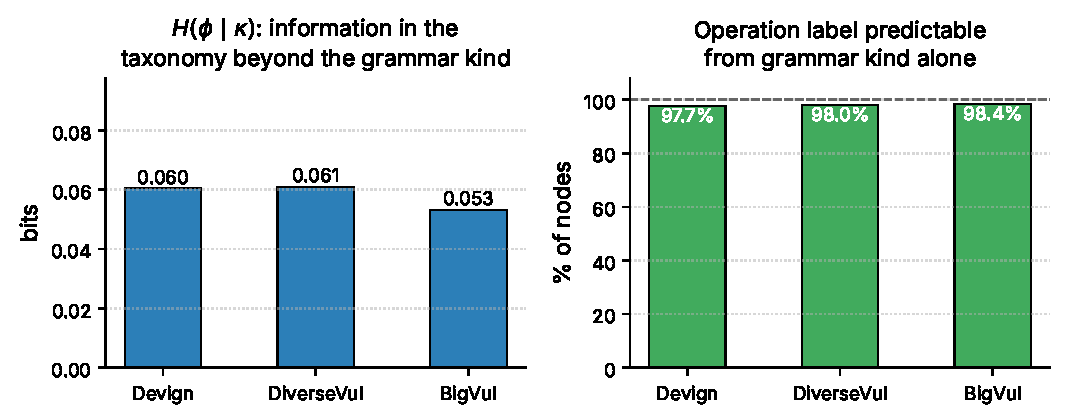
\includegraphics[width=\linewidth]{fig_redundancy.pdf}
\caption{The information the taxonomy carries beyond the grammar kind,
$H(\phi \mid \kappa)$ (left), and the share of nodes whose operation label is
recoverable from the kind alone (right)}
\label{fig:redundancy}
\end{figure}

\textbf{The taxonomy adds almost nothing to the kind.} $H(\phi \mid \kappa)$
lies between \numhPhiGivenKindMin{} and \numhPhiGivenKindMax{} bits on the
three corpora (Table~\ref{tab:rq2b_information} and Figure~\ref{fig:redundancy}); between \numdeterminismMin\% and \numdeterminismMax\% of nodes have an operation
label that is fixed by the node kind (\numbigvulDeterminism\% on BigVul). This
follows from the definition rather than from an accident of the data: rules~2
and~3 of Section~\ref{sec:phi} are decided by the node kind or its operator
token, so for most kinds $\phi$ is a constant function of $\kappa$. Only
call expressions (is this callee a memory operation?) and binary expressions
(which operator?) carry residual uncertainty.

\textbf{The taxonomy discards much of the kind.} $H(\kappa \mid \phi)$ is
\numbigvulHKindGivenPhi{} bits on BigVul, \numbigvulKindLost\% of the kind's
entropy: collapsing 364 kinds into nine operation types throws away about two
thirds of what the kind alphabet distinguishes. So $\phi$ is not a neutral
re-encoding of $\kappa$; it is a lossy compression, and an abstraction in that
position cannot be expected to outperform its source.

These are properties of two deterministic labelling functions over a joint
table of $|\mathcal{T}_8| \times |K|$ cells, so they converge quickly: the
bootstrap intervals over functions in Table~\ref{tab:rq2b_information} are
at most \numkindGivenPhiCiWidthMax{} bits wide. The diagnostic costs minutes, needs no training, and
would have predicted the experimental pattern of the next sections from the
definition of $\phi$ alone. We offer it as a reusable check for anyone who
proposes an engineered abstraction over a parse tree: compute
$H(\text{abstraction} \mid \text{grammar kind})$ and $H(\text{grammar kind}
\mid \text{abstraction})$ before crediting the abstraction with an effect.


\subsection{RQ3: generality across corpora and architectures}
\label{sec:rq_generality}

\emph{In short:} the benefit of dropping project vocabulary holds on both
corpora and under every architecture we tried (the Transformer on BigVul
only); the choice of architecture
moves AUC by much less than the choice of node view, but only within the
family of small models we can train from scratch.

Table~\ref{tab:rq3_generality} repeats the main comparison on DiverseVul and
under three further architectures: GAT and GIN (two other message-passing
schemes) and a Transformer encoder over the pre-order node sequence, which uses
no graph edges at all (BigVul only, for cost). Figure~\ref{fig:forest} plots
the gains against the text-only view.


\begin{tableorg}[t]
\centering
\caption{RQ3: mean AUC over 10 matched folds for four node views under every
backbone and corpus, and the paired gain of $\kappa$ and of lexical$+\kappa$
over the lexical view (point estimate, 95\% cluster-bootstrap interval,
bootstrap $p$; \emph{n.s.}: interval contains zero).}
\label{tab:rq3_generality}
\adjustbox{max width=\textwidth}{%
\begin{tabular}{llrrrrll}
\toprule
Corpus & Backbone & Lexical & Lex$+\kappa$ & $\kappa$ & $\kappa{+}\phi$ & $\kappa$ vs lexical & Lex$+\kappa$ vs lexical \\
\midrule
BigVul & GGNN & 0.506 & 0.592 & 0.691 & 0.687 & $+0.185$ $[+0.130, +0.236]$ $<0.001$ & $+0.086$ $[+0.038, +0.111]$ $<0.001$ \\
BigVul & GAT & 0.507 & --- & 0.673 & 0.654 & $+0.167$ $[+0.117, +0.227]$ $<0.001$ & --- \\
BigVul & GIN & 0.574 & --- & 0.704 & 0.719 & $+0.131$ $[+0.089, +0.197]$ $<0.001$ & --- \\
BigVul & Transformer & 0.582 & --- & 0.706 & --- & $+0.124$ $[+0.088, +0.166]$ $<0.001$ & --- \\
DiverseVul & GGNN & 0.566 & 0.607 & 0.667 & 0.675 & $+0.101$ $[+0.070, +0.132]$ $<0.001$ & $+0.042$ $[+0.021, +0.061]$ $<0.001$ \\
DiverseVul & GAT & 0.558 & --- & 0.652 & 0.654 & $+0.094$ $[+0.060, +0.127]$ $<0.001$ & --- \\
DiverseVul & GIN & 0.574 & --- & 0.679 & 0.687 & $+0.105$ $[+0.069, +0.136]$ $<0.001$ & --- \\
\bottomrule
\end{tabular}}
\end{tableorg}

\begin{figure}[t]
\centering
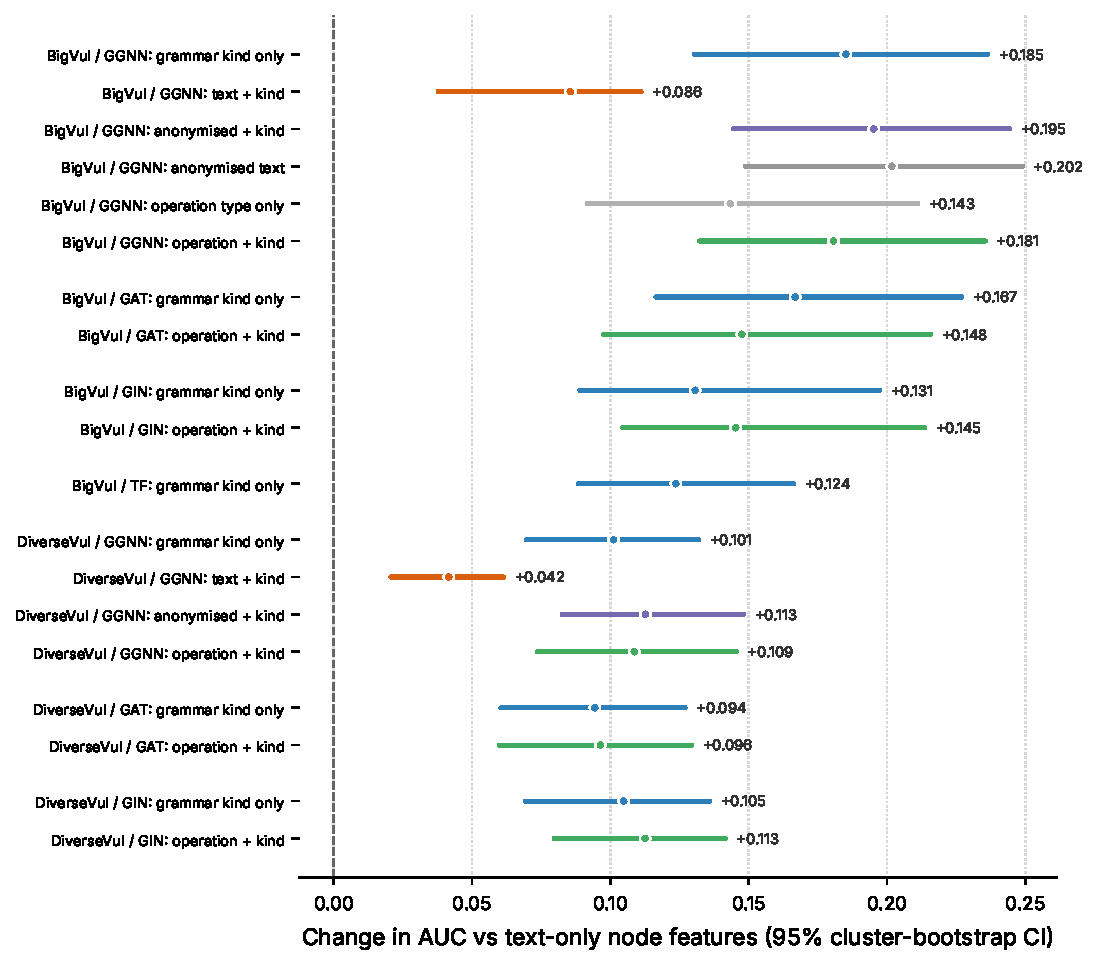
\includegraphics[width=\linewidth]{fig_representation_forest.pdf}
\caption{Change in AUC against text-only node features for each corpus and
architecture, with 95\% cluster-bootstrap intervals over held-out projects.
Intervals that include zero would be marked n.s}
\label{fig:forest}
\end{figure}

\paragraph{Corpora and message-passing schemes} Under GAT and GIN, and on
DiverseVul, the grammar kind improves on text in every comparison
(Table~\ref{tab:rq3_generality}; for example
\cDvGgnnKindVLexD{} on DiverseVul with the GGNN, \cDvGatKindVLexD{} with the
GAT and \cDvGinKindVLexD{} with the GIN). The gain varies by corpus
(\cBvGgnnKindVLexD{} on BigVul with the GGNN, against \cDvGgnnKindVLexD{} on
DiverseVul).

\paragraph{The architecture claim, narrowed} The earlier submission asserted
that representation matters more than architecture on the strength of three
message-passing networks whose AUCs differed by $0.027$. That evidence cannot
support a claim about architecture in general, and we now state what it does
support. Under a fixed vocabulary-free view the three message-passing
networks (GGNN, GAT, GIN) span \numbvSpreadKind{} AUC on BigVul with the
grammar kind and \numdvSpreadKind{} on DiverseVul; under the text view they
span \numbvSpreadLex{} and \numdvSpreadLex{}. The widest of these ranges is
smaller than the smallest gain of any vocabulary-free view over text
(\numdeltaMin{}), so within this family the node view is a larger lever than
the backbone. The Transformer adds a different inductive bias (no edges); its
AUC is \mBvTfLexAuc{} with text and \mBvTfKindAuc{} with the grammar kind, so
the benefit of the vocabulary-free view is not specific to message passing.
What our evidence cannot show is that no \emph{pretrained} or much larger
architecture would close the gap by itself, and Section~\ref{sec:rq_reference}
shows that a fine-tuned pretrained code model, reading format-normalised source,
beats the vocabulary-free graph views by a small margin.


\subsection{RQ4: ablations}
\label{sec:rq_ablation}

We remove one component at a time under the grammar-kind view on BigVul (GGNN,
the same 10 folds as before) and report the paired change in AUC
(Table~\ref{tab:ablation}). Beyond the node views of Table~\ref{tab:direct},
which already ablate the contribution of text, anonymisation, kind and
operation type, two structural components are examined.

\paragraph{Edge types} Removing the def-use edges changes AUC by
\numedgeNoDuDiff{} (\numedgeNoDuLo{} to \numedgeNoDuHi{}); keeping only the
syntax-tree edges changes it by \numedgeAstOnlyDiff{} (\numedgeAstOnlyLo{} to
\numedgeAstOnlyHi{}). These measure the contribution of the data-flow
approximation, and of source order together with it, on top of the tree.
Neither changes AUC measurably under the grammar-kind view: the network gets
little from the approximate def-use and ordering edges beyond the tree itself. (A
variant that removes only the sibling-order edges was dropped from the grid
for cost.)

\paragraph{Operation-alphabet granularity} Refining $\phi$ from eight to
sixteen operation types changes AUC by \numgranTOneSixDiff{}
(\numgranTOneSixLo{} to \numgranTOneSixHi{}) over \numgranTOneSixFolds{} matched
folds. The first submission reported a thirty-two-type run that rested on a
single fold; the claim that granularity does not matter was not supported by
that run and we do not repeat it. The one measurement we do have is consistent
with a null, as expected from Section~\ref{sec:rq_why}, since the classes that a
finer alphabet separates are rare: the memory-operation class fires on only
\numbvMemoryPct\% of nodes (Table~\ref{tab:node_dist}). The thirty-two-type
refinement was not re-run for this version because of its cost, so we make no
statement about it.


\begin{tableorg}[t]
\centering
\caption{Ablations on BigVul (GGNN). First block: removing edge types from the
graph under the $\kappa$ view. Second block: refining the operation alphabet
under the $\kappa{+}\phi$ view, compared against the same view at
$|\mathcal{T}|=8$ on the same folds. $\Delta$AUC is paired, with 95\%
cluster-bootstrap interval and bootstrap $p$.}
\label{tab:ablation}
\adjustbox{max width=\textwidth}{%
\begin{tabular}{lrrl}
\toprule
Variant & Folds & AUC & $\Delta$AUC vs reference [95\% CI] $p$ \\
\midrule
All edges (AST+SIB+DU), $\kappa$ & 10 & 0.691 & --- \\
\quad no def-use edges & 10 & 0.691 & $+0.000$ $[-0.012, +0.019]$ 0.758\,n.s. / 1.000 \\
\quad AST edges only & 10 & 0.699 & $+0.008$ $[-0.009, +0.027]$ 0.330\,n.s. / 0.375 \\
$\kappa{+}\phi$ with $|\mathcal{T}|=16$ vs $8$ & 10 & 0.691 & $+0.004$ $[-0.022, +0.019]$ 0.920\,n.s. / 0.625 \\
\bottomrule
\end{tabular}}
\end{tableorg}


\subsection{RQ5: reference points}
\label{sec:rq_reference}

Table~\ref{tab:baselines} places our views next to re-implementations of the
\emph{input representations} used by existing approaches, a pretrained code
model, and the trivial size rule, all on the same samples and folds.
They are not reproductions of the published systems or their published numbers,
which use different data splits and often within-project evaluation.


\begin{tableorg}[t]
\centering
\caption{Comparison with existing approaches re-implemented under the same
sample, folds and metrics (mean $\pm$ std over 10 project-level folds). These
are re-implementations of the \emph{input representation} of each approach
inside one training protocol, not reproductions of the published systems or
their published numbers. UniXcoder rows use a frozen encoder and a linear
probe. \emph{Format-normalised} source is the parser's token stream with
whitespace and comments removed (Section~\ref{sec:artefact}). The last three
rows score functions without reading what the code says.}
\label{tab:baselines}
\adjustbox{max width=\textwidth}{%
\begin{tabular}{lcccc}
\toprule
 & \multicolumn{2}{c}{BigVul} & \multicolumn{2}{c}{DiverseVul} \\
System & AUC & AUPRC & AUC & AUPRC \\
\midrule
GGNN on code text (token-only baseline) & 0.506 $\pm$ 0.077 & 0.085 $\pm$ 0.034 & 0.566 $\pm$ 0.039 & 0.080 $\pm$ 0.017 \\
Devign/ReVeal-style GGNN: text $+$ node type & 0.592 $\pm$ 0.072 & 0.105 $\pm$ 0.039 & 0.607 $\pm$ 0.027 & 0.096 $\pm$ 0.024 \\
GGNN, anonymised tokens $+$ node type & 0.701 $\pm$ 0.059 & 0.180 $\pm$ 0.059 & 0.679 $\pm$ 0.036 & 0.122 $\pm$ 0.030 \\
Transformer over node sequence, text & 0.582 $\pm$ 0.074 & 0.106 $\pm$ 0.042 & --- & --- \\
Transformer over node sequence, $\kappa$ & 0.706 $\pm$ 0.039 & 0.155 $\pm$ 0.041 & --- & --- \\
Pretrained UniXcoder, frozen, linear probe (raw source) & 0.705 $\pm$ 0.061 & 0.163 $\pm$ 0.035 & 0.623 $\pm$ 0.027 & 0.095 $\pm$ 0.022 \\
Pretrained UniXcoder, frozen, linear probe (format-normalised) & 0.645 $\pm$ 0.069 & 0.109 $\pm$ 0.022 & 0.604 $\pm$ 0.015 & 0.088 $\pm$ 0.019 \\
LineVul-style: fine-tuned CodeBERT (raw source) & 0.922 $\pm$ 0.026 & 0.748 $\pm$ 0.063 & 0.693 $\pm$ 0.028 & 0.123 $\pm$ 0.026 \\
LineVul-style: fine-tuned CodeBERT (format-normalised) & 0.728 $\pm$ 0.058 & 0.189 $\pm$ 0.058 & 0.705 $\pm$ 0.028 & 0.131 $\pm$ 0.023 \\
No code read: function size (node count) & 0.736 $\pm$ 0.065 & 0.232 $\pm$ 0.087 & 0.715 $\pm$ 0.028 & 0.152 $\pm$ 0.028 \\
No code read: trailing-whitespace rule & 0.830 $\pm$ 0.050 & 0.392 $\pm$ 0.109 & 0.542 $\pm$ 0.024 & 0.069 $\pm$ 0.018 \\
No code read: gradient boosting on formatting statistics & 0.896 $\pm$ 0.026 & 0.601 $\pm$ 0.065 & 0.634 $\pm$ 0.033 & 0.111 $\pm$ 0.034 \\
GGNN, grammar kind $\kappa$ (ours) & 0.691 $\pm$ 0.037 & 0.149 $\pm$ 0.027 & 0.667 $\pm$ 0.021 & 0.105 $\pm$ 0.026 \\
GGNN, $\kappa{+}\phi$ (ours) & 0.687 $\pm$ 0.060 & 0.158 $\pm$ 0.042 & 0.675 $\pm$ 0.021 & 0.114 $\pm$ 0.030 \\
\bottomrule
\end{tabular}}
\end{tableorg}

\paragraph{Devign/ReVeal-style input} Text together with the node type
(\texttt{lex+$\kappa$} with a GGNN) reaches AUC \mBvGgnnLexKindAuc{} on BigVul
and \mDvGgnnLexKindAuc{} on DiverseVul, which is below the grammar-kind and anonymised views in
Table~\ref{tab:rq2_representation}.

\paragraph{Pretrained code models: read the format-normalised rows} Table~\ref{tab:baselines}
holds two pretrained references: UniXcoder~\citep{guo2022unixcoder} with a frozen
encoder (its weights are not updated; it turns each function into one vector) and
a linear probe (a logistic regression trained on that vector), and a
LineVul-style detector~\citep{fu2022linevul}, that is, CodeBERT fine-tuned
end to end on the function text (function-level classifier only; three epochs,
the same class-weighted loss and folds as every other system, run on a rented
GPU). On raw source they reach AUC \numbvUnixAuc{} and \rBvLinevulAuc{} on BigVul,
\numdvUnixAuc{} and \rDvLinevulAuc{} on DiverseVul. On BigVul those figures partly
measure the formatting artefact of Section~\ref{sec:artefact}, so the fair
comparison uses format-normalised source, where the same two systems reach
\rBvUnixNormAuc{} and \rBvLinevulNormAuc{} (BigVul) and \rDvUnixNormAuc{} and
\rDvLinevulNormAuc{} (DiverseVul). Against these normalised references the
vocabulary-free graph networks are better than the frozen probe (GGNN with
$\kappa$: \cBvGgnnKindVUnixNormD{} on BigVul, \cBvGgnnKindVUnixNormLo{} to
\cBvGgnnKindVUnixNormHi{}; \cDvGgnnKindVUnixNormD{} on DiverseVul) and below the
fine-tuned model by a small margin (\cBvGgnnKindVLinevulNormD{},
\cBvGgnnKindVLinevulNormLo{} to \cBvGgnnKindVLinevulNormHi{} on BigVul;
\cDvGgnnKindVLinevulNormD{}, \cDvGgnnKindVLinevulNormLo{} to
\cDvGgnnKindVLinevulNormHi{} on DiverseVul). Two lessons follow. First, ``text
hurts cross-project transfer'' is a statement about token embeddings learned
from scratch on a few thousand functions, not about text in general: a model that
has seen billions of code tokens before, and is fine-tuned, uses identifiers and
beats our graph models by about 0.04 AUC. Second, that margin is small in
absolute terms: the fine-tuned model is not distinguishable from the
function-size rule (BigVul \xBvLinevulNormVSizeD{}, \xBvLinevulNormVSizeLo{} to
\xBvLinevulNormVSizeHi{}; DiverseVul \xDvLinevulNormVSizeD{}).

\paragraph{A size rule beats every network} Scoring a function by its node
count alone gives AUC \numbvSizeAuc{} (BigVul) and \numdvSizeAuc{} (DiverseVul),
a higher mean AUC than any network in this study. (On BigVul a formatting-only
classifier is higher still; Section~\ref{sec:artefact}.) The paired differences are significant under
the project-cluster bootstrap for most networks (e.g.\ $\kappa$ with the GGNN
against size: \cBvGgnnKindVSizeD{}, \cBvGgnnKindVSizeLo{} to
\cBvGgnnKindVSizeHi{} on BigVul) but not for all (for example the GIN with
$\kappa{+}\phi$ on BigVul). We read this as a caution about the whole
benchmark family: under project-disjoint evaluation, much of what these
corpora reward is a length prior, and absolute AUCs of $0.6$ to $0.7$ should not
be read as evidence of vulnerability understanding.


\subsection{A formatting artefact in BigVul, and what it does to models that read text}
\label{sec:artefact}

\emph{In short:} in BigVul, the raw formatting of a function tells whether it is
labelled vulnerable, almost independently of what the code does. A model that
reads source text can use this; our graph models cannot, because the parser
discards formatting.

\paragraph{How it was found.} We fine-tuned a LineVul-style detector
(CodeBERT~\citep{fu2022linevul} fine-tuned on the raw function text, on a GPU
rented for the purpose, with the same ten project-level folds) as the stronger
pretrained reference that reviewers of an earlier version asked for. It scored
a mean AUC of \rBvLinevulAuc{} on BigVul (AUPRC \rBvLinevulAuprc{}), far above
every graph model, which is implausible for cross-project detection and
prompted a search for a shortcut.

\paragraph{The artefact.} \numartBvTrailVuln\% of the vulnerable BigVul functions
in our sample contain at least one line that ends in trailing whitespace,
against \numartBvTrailBenign\% of the benign functions. In DiverseVul the
corresponding figures are \numartDvTrailVuln\% and \numartDvTrailBenign\%.
Two baselines that never read what the code says expose the consequence
(Table~\ref{tab:baselines}, last rows). A single rule that scores a function by
the fraction of its lines with trailing whitespace reaches AUC \rBvTrailAuc{}
on BigVul (\rDvTrailAuc{} on DiverseVul); gradient boosting over sixteen
formatting and size statistics (length, number of lines, tabs, carriage
returns, trailing whitespace, blank lines, comment markers, indentation, and so
on) reaches \rBvFormatAuc{} (\rDvFormatAuc{} on DiverseVul), on the same
project-disjoint folds. The first is above every graph model in this study; the
second is above all of them by a wide margin. We do not know why the corpus
carries this signal (a plausible cause is that benign functions pass through a
different extraction or formatting step than vulnerable ones), only that it is
present, strong, and project-independent.

\paragraph{Removing it.} We re-run the text-reading systems on
\emph{format-normalised} source: the parser's token stream with comments
dropped and every token separated by one space, so indentation, line breaks,
trailing whitespace, tabs and comments are gone while identifiers, literals and
operators are unchanged (\numartBvTrailNormAny\% of normalised functions contain
trailing whitespace). Table~\ref{tab:baselines} shows that fine-tuned CodeBERT
falls from \rBvLinevulAuc{} on raw BigVul source to \rBvLinevulNormAuc{} on
normalised source (paired difference \xBvLinevulVLinevulNormD{}, 95\% interval
\xBvLinevulVLinevulNormLo{} to \xBvLinevulVLinevulNormHi{}; AUPRC from
\rBvLinevulAuprc{} to \rBvLinevulNormAuprc{}), and the frozen UniXcoder probe from
\rBvUnixAuc{} to \rBvUnixNormAuc{} (\xBvUnixVUnixNormD{}). On DiverseVul, where the
artefact is much weaker, the corresponding falls are from \rDvLinevulAuc{} to
\rDvLinevulNormAuc{} and from \rDvUnixAuc{} to \rDvUnixNormAuc{}. Even after
normalisation, fine-tuned CodeBERT reaches only \rBvLinevulNormAuc{} on BigVul
and \rDvLinevulNormAuc{} on DiverseVul, against \numbvSizeAuc{} and
\numdvSizeAuc{} for the function-size rule (BigVul paired difference
\xBvLinevulNormVSizeD{}, \xBvLinevulNormVSizeLo{} to \xBvLinevulNormVSizeHi{}): a
fine-tuned 125-million-parameter model reading the identifiers does not clearly
beat a count of syntax-tree nodes.

\paragraph{What this means for the rest of the paper.} First, the graph models
are not affected: the grammar kind, the anonymised and the operation views are
computed from the parse tree, which contains no formatting, so the comparisons of
Sections~\ref{sec:rq_representation}--\ref{sec:rq_ablation} stand. The
function-size rule and the size-binned AUC are likewise unaffected, since node
count does not depend on formatting. Second, the pretrained references of
Section~\ref{sec:rq_reference} must be read on normalised source, not raw: on
raw BigVul source they partly measure formatting. Third, for the field, any
result on BigVul from a model that reads raw text, including the large
pretrained models, should be checked against a formatting-only baseline before it
is attributed to an understanding of the code. We have not audited published
results and make no claim about them; the check costs one line of code per
corpus.


\subsection{Summary of findings}
\label{sec:summary}

\begin{enumerate}
    \item \textbf{Text read from scratch fails across projects.} AUC is
          \mBvGgnnLexAuc{} (BigVul) and \mDvGgnnLexAuc{} (DiverseVul), close to
          random.
    \item \textbf{Removing project vocabulary helps by about \numdeltaMin{} to \numdeltaMax{} AUC,}
          on both corpora and under every architecture we ran (the Transformer on
          BigVul only), whether it is removed
          by anonymising identifiers or by using the grammar kind.
    \item \textbf{The grammar kind does not beat anonymised text;} its advantage
          is that it needs no preprocessing decision.
    \item \textbf{The engineered operation taxonomy adds nothing} to the grammar
          kind, and the reason is measurable: it is almost a function of it
          (Section~\ref{sec:rq_why}). As a static analysis it is accurate for the
          question it answers (memory operation or not: precision
          \numpooledMemopP{}, recall \numpooledMemopR{}) but less accurate than
          first reported at the level of individual classes.
    \item \textbf{Much of that gain is about function size.} Within bins of
          function size the gain over text is not distinguishable from zero for
          the grammar kind in every corpus--architecture cell we ran, and within-bin AUC is \mBvGgnnKindSs{} (BigVul) and
          \mDvGgnnKindSs{} (DiverseVul).
    \item \textbf{Classifiers that read no code beat every network:} a
          one-line size rule on both corpora and, on BigVul, a classifier on
          formatting statistics alone (AUC \rBvFormatAuc{}), because the corpus
          has a formatting artefact. Models that read raw text partly exploit
          it (Section~\ref{sec:artefact}). Absolute performance of the graph
          models is weak.
\end{enumerate}


\section{Discussion}
\label{sec:discussion}

\subsection{What the evidence supports}
Four statements survive every control we ran. First, a graph network that
learns embeddings of project-specific text from scratch transfers to new
projects barely better than chance. Second, any description of nodes that does
not contain that vocabulary does substantially better, by roughly \numdeltaMin{} to \numdeltaMax{}
AUC, on both corpora and under every architecture we ran. Third, among the
vocabulary-free descriptions the differences are small: renaming identifiers is
about as good as the grammar kind, and an engineered operation taxonomy adds
nothing to the grammar kind. Fourth, much of the gap between text and the
vocabulary-free views is a gap in representing function size: within size bins
the grammar kind is not distinguishable from text, and on DiverseVul no GGNN view is.
The first two statements are consistent with a simple account: a lexical model's input at test time is largely out-of-vocabulary, and
the part that is in vocabulary correlates with project identity rather than with
the weakness. We have not isolated the mechanism experimentally (for instance
by varying the out-of-vocabulary rate while holding everything else fixed), so
this remains an interpretation.

\subsection{What it does not show}
The results do not show that grammar kinds, or any node description, make
vulnerability detection work across projects. A rule that ranks functions by
their node count beats every network in the study (Section~\ref{sec:rq_reference}),
and on BigVul a classifier that sees only formatting beats all of them
(Section~\ref{sec:artefact}),
and the gains of the vocabulary-free views over text largely vanish within
bins of function size (Section~\ref{sec:rq_representation}). Nor do they
show that text is harmful in general: a fine-tuned pretrained code model reading
format-normalised source beats the graph models by a small margin
(Section~\ref{sec:rq_reference}). The honest reading is that the
standard from-scratch lexical baseline of graph-based detectors is weak under
project-disjoint evaluation, so improvements over it are cheap and should be
compared with the stronger baselines listed above.

\subsection{Evaluating an abstraction before crediting it}
For a languages audience the methodological point is the more portable one. A
proposed abstraction over a parse tree should be examined on two fronts that
are rarely both reported. As a program analysis, it should be scored against
annotated ground truth with agreement and uncertainty reported, as in
Section~\ref{sec:rq_analysis}; the first version of this work did that with a
single, non-blind annotator and reported an accuracy higher than the blind
protocol supports. As a representation, it should be compared with the parser's
own alphabet through the two conditional entropies of Section~\ref{sec:rq_why},
which cost minutes and would have predicted our null from the definition of the
abstraction. A third check is cheap and is the one we most nearly omitted: ask
whether a function-length rule does as well.

\subsection{Threats to validity and limitations}
\label{sec:limitations}

\textbf{Graph fidelity.} Our graphs are tree-sitter syntax trees with sibling and
approximate def-use edges, not Code Property Graphs. Every compared system
consumes the same graph, so the comparison is internally fair, but absolute
performance is bounded by this choice and conclusions may differ with richer
graphs.

\textbf{Sample, truncation and length.} Each corpus is a uniform random sample
of about 10{,}000 functions (roughly \numbigvulVuln{} and \numdiversevulVuln{}
vulnerable functions). The 200-node cap truncates a quarter or fewer of
functions overall but far more of the vulnerable ones (Table~\ref{tab:corpora}),
so what lies beyond the cap is invisible to every system. Because vulnerable
functions are longer, any detector may partly learn length; we measured this
rather than removing it.

\textbf{Training budget and tuning.} Every system trains for the same fixed
number of epochs with hyper-parameters chosen in advance and not tuned on any
fold (Table~\ref{tab:hparams}). A longer or tuned schedule could change absolute
numbers, in particular for the lexical view, although fixing the budget across
views is what makes the comparison controlled. Each fold uses a single
initialisation seed shared across systems, so run-to-run variance within a fold
is not estimated; the paired tests treat folds, not seeds, as the unit.

\textbf{Dependence between folds.} Folds from the second repeat reuse some test
projects of the first, so the ten folds are not independent. The cluster
bootstrap resamples projects and the Wilcoxon test is reported alongside it, but
the effective sample size is smaller than ten.

\textbf{Annotation.} The callee validation uses two blind annotators and a
third pass on disagreements, but all three are language models; no human
labelled the sheets. The original, single-annotator labels agree with the new
consensus at Cohen's $\kappa$ of \numdevignOrigKappa{}. A human second
annotator remains desirable, and the released sheets allow one to be added.
Several classes have few positive names, so their intervals are wide.

\textbf{Label noise and language.} We inherit the labels of the corpora, whose
accuracy is contested in the literature that produced them, and we study C only.

\textbf{Pretrained references.} The fine-tuned model reproduces only the
function-level classifier of LineVul, for three epochs, without checkpoint
selection; the UniXcoder result is a frozen encoder with a linear probe on 256
tokens. Longer or tuned schedules, or larger models, could score higher.

\textbf{Earlier claims withdrawn.} The first submission also reported federated
and privacy experiments and a learned edge mask. They are not part of this
work, and nothing here supports or refutes them.


\section{Conclusion}
\label{sec:conclusion}

We asked how much of the cross-project failure of graph-based vulnerability
detectors depends on what a node is told about the code. Under a controlled,
project-disjoint protocol with ten matched folds, node descriptions that contain
a project's vocabulary performed close to chance, while descriptions that do
not (renamed identifiers, or the parser's grammar kinds) performed better by
roughly \numdeltaMin{} to \numdeltaMax{} AUC on two corpora and every architecture we ran. They performed
about equally well, and the hand-built operation taxonomy that we expected to
help added nothing to the grammar kind. We explained that null exactly: the
taxonomy is \numdeterminismMin{}--\numdeterminismMax{}\% determined by the kind, depending on the corpus.

The same controls also limit the result. A rule that scores a function by its
length has a higher mean AUC than every network we trained, on BigVul a
classifier that reads only formatting does better still, the gain over text largely
disappears within bins of function size, a fine-tuned pretrained model beats the graph views by only a small margin
once formatting is removed, and the labelling function is less accurate class by class than
our first, non-blind validation suggested. We therefore recommend that studies
of learned vulnerability detectors report a function-size baseline and a
vocabulary-free baseline next to any new architecture or representation, and
that proposed abstractions over a parse tree be checked against the grammar
alphabet before they are credited with an effect. Cross-project vulnerability
detection from small, from-scratch models remains an open problem.


\section*{Declarations}

\begin{itemize}
\item \textbf{Funding:} This research did not receive any specific grant from funding agencies in the public, commercial, or not-for-profit sectors.
\item \textbf{Conflict of interest/Competing interests:} The author has no relevant financial or non-financial interests to disclose.
\item \textbf{Ethics approval and consent to participate:} Not applicable. The study uses publicly available source-code corpora and involves no human participants.
\item \textbf{Consent for publication:} Not applicable.
\item \textbf{Data availability:} The study uses the public corpora BigVul, DiverseVul and Devign, accessed through the public mirrors named in the text. The sampled function identifiers, the per-fold held-out predictions of every system, and the annotation sheets are in the repository below.
\item \textbf{Materials availability:} Not applicable.
\item \textbf{Code availability:} All code, annotation sheets and the scripts that regenerate every table, figure and number in this paper are available at \url{https://github.com/vinhqdang/vulmorph-fed}.
\item \textbf{Author contribution:} Single author.
\item \textbf{Use of large language models:} Language models were used as the two blind annotators and the adjudicator in the validation of Section~\ref{sec:rq_analysis}, as described there. Language-model assistants also helped with writing code and drafting text; the author reviewed and edited all content and takes full responsibility for it.
\end{itemize}

\bibliography{ref}

\end{document}
